\documentclass[12pt]{article}

%% Language and font encodings
\usepackage[english]{babel}
\usepackage[utf8x]{inputenc}
\usepackage[T1]{fontenc}

%% Sets page size and marginsp
\usepackage[letterpaper,top=3cm,bottom=2cm,left=3cm,right=3cm,marginparwidth=1.75cm]{geometry}

%% Spacing
\usepackage{setspace}
%\doublespacing
\onehalfspacing

%% Useful packages
\usepackage{amsmath}
\usepackage{amssymb}
\usepackage{graphicx}
\usepackage[colorinlistoftodos]{todonotes}
\usepackage[colorlinks=true, allcolors=blue]{hyperref}
\usepackage{amsthm}
\usepackage{lscape}
\usepackage{thmtools}
\usepackage{thm-restate}

%% for tables
\usepackage{booktabs,caption}
\usepackage[flushleft]{threeparttable}
\usepackage{multirow}
\usepackage{siunitx}

% for placing figures
\usepackage{float}
%\usepackage[nolists,tablesfirst]{endfloat}

% citations
\usepackage[]{natbib}

% appendices
\usepackage[toc,page]{appendix}

% Custom definitions
\def\bmath#1{\mbox{\boldmath$#1$}}
\def\sym#1{\ifmmode^{#1}\else\(^{#1}\)\fi}
\declaretheorem[name=Theorem,numberwithin=section]{theorem}
\declaretheorem[name=Proposition,numberwithin=section]{proposition}
\declaretheorem[name=Lemma,numberwithin=section]{lemma}
\declaretheorem[name=Corollary,numberwithin=section]{corollary}
\declaretheorem[name=Definition,numberwithin=section]{definition}

%for to do bubbles
\usepackage[colorinlistoftodos]{todonotes}

%for highlighting
\usepackage{soul}

%for including pdfs
\usepackage{pdfpages}

%%%%%%%%%%%%%%%%%%%%%%%%%%%%%%%%%%%%%%%%%%%%%%%%%%%%%
\title{{\bf Experiments in High-Frequency Trading: \\ Comparing Two Market Institutions}
\thanks{This project received funding from the Center for Analytical Finance (CAFIN) at the University of California, Santa Cruz and from the European Research Council (ERC) under the European Union's Horizon 2020 research and innovation programme (grant agreement No 741409). 
This paper is part of a larger, joint project with Dan Friedman, Axel Ockenfels, Peter Cramton. We thank them for invaluable feedback and Darrel Hoy and David Malec for developing the remote exchanges. 
We thank conference and seminar audiences at: the 2016 SEF meeting in Tucson, the 2017 SEF meeting in Nice (in particular, J{\"u}rgen Huber, Peter Bossaerts and Stefan Palan), the 2017 ESA meeting in Richmond, ICESI University, the UCSC-Econ brown bag seminar, the 2018 CAFIN HFT workshop (in particular, Pete Kyle). 
% EA: do you agree with thanking Kyle like this?
We also thank  Morgan Grant, Jason Vranek and Daniel Thurau for excellent programming work at the UCSC LEEPS Laboratory.
The results reflect the authors' view -- the ERC is not responsible for any use that may be made of the information it contains.}}
\author{
  Eric M. Aldrich\thanks{
  Email: ealdrich@ucsc.edu.} \\
  \normalsize{Department of   Economics} \\
  \normalsize{University of California, Santa Cruz}
\and
  Kristian López Vargas\thanks{
  Email: kristian@ucsc.edu.} \\
  \normalsize{Department of Economics} \\
  \normalsize{University of California, Santa Cruz}
}

\begin{document}

\renewcommand{\baselinestretch}{1}

\date{June 16, 2018}

\maketitle

\vspace{-.25in}

\begin{abstract}
We implement a laboratory financial market where traders can access costly technology that reduces communication latency with a remote exchange. In this environment, we conduct a market design study on high-frequency trading: we contrast the performance of the newly proposed Frequent Batch Auction (FBA) against the Continuous Double Auction (CDA), which organizes trades in most exchanges worldwide. Our evidence suggests that, relative to the CDA, the FBA exhibits (1) less predatory trading behavior, (2) lower investments in low-latency communication technology, (3) lower transaction costs, and (4) lower volatility in market spreads and liquidity. We also find that transitory shocks in the environment have substantially greater impact on market dynamics in the CDA than in the FBA.
\end{abstract}

\noindent \textbf{Keywords:} Market design, Auctions, High-Frequency Trading, Continuous Double Auction, Frequent Batch Auction.

\noindent \textbf{JEL Classification:} C91, D44, D47, D53, G12, G14.

\renewcommand{\baselinestretch}{2}

\newpage

\section{Introduction \label{Intro}}

Telecommunications technology has transformed financial markets in the last decade. Order submission and execution times at major exchanges have declined from seconds to microseconds (1 millionth of a second). As a consequence, traders are rewarded for reacting quickly to information, resulting in a new market participant: high-frequency trading (HFT) firms. HFT firms use computerized strategies to transact large volumes in fractions of a second and now account for more than half of transactions at major exchanges worldwide. 
% for later: let us have a source for the previous claim.
Proponents claim that HFT has improved market liquidity (the ease with which trades can occur) and reduced transaction costs \citep{Narang2010}. Opponents argue that the multi-billion-dollar cost of HFT infrastructure is ultimately borne by investors, its liquidity is illusory, and it is a destabilizing force in financial markets \citep{Lewis2015}. 

Most academic papers studying HFT use proprietary data with trader identification, and are able to classify accounts as either aggressive (primarily liquidity consuming) or passive (primarily liquidity providing). Passive accounts are almost uniformly associated with improved market performance. \cite{Hagstromer2013, Malinova2014, Brogaard2015b, Jovanovic2015} and \cite{Menkveld2017} are examples of papers that find such positive effects.
The effects of aggressive HFT, however, are mixed: it is generally associated with informed price impact over short horizons, increased adverse selection costs for other traders, increased short-term volatility, and higher trading costs for institutional and retail traders. Examples from this literature include \cite{Zhang2011, Bershova2012, Breckenfelder2013, Brogaard2013,  Hasbrouck2013,  Hendershott2013, Hirschey2013, Baldauf2015, Baldauf2015a, Brogaard2015a} and \cite{Menkveld2017}.

Despite the uncertainty surrounding the effects of high-speed trading, policy makers worldwide are already taking actions intended to discourage HFT. For example, in 2016, the U.S. Securities and Exchange Commission approved the Investors Exchange (IEX) to operate as a public securities exchange. A primary goal of the IEX market, which was founded in 2012 to provide a non-public alternative trading system (ATS) with delayed messaging \citep[see][]{Aldrich2017}, is to reduce potential advantages of HFT firms. The SEC decision to approve the IEX system as a public exchange had substantial network effects, primarily because of quote protection under Reg NMS Rule 611 \citep{Hu2018}. In addition to IEX, several other market formats have been proposed as alternatives to the CDA. These include the frequent batch auction (\cite{Budish2015}, \cite{Budish2014}) and the fully continuous exchange \citep{Kyle2017}. However, no scientific evidence exists on the relative performance of such market institutions.

The objective of this paper is not to address the net costs or benefits of HFT, but instead to compare the effects of different trading environments on market quality in the presence of HFT. Specifically, we use laboratory experiments to compare two leading financial market formats in the presence of high-frequency trading: the continuous double auction (CDA) and the frequent batch auction (FBA). The CDA (also known as the continuous limit order book) organizes trade in the majority of equities, futures and currency exchanges around the world. In this format, traders make publicly committed offers to buy and sell assets and are able to accept others’ offers at any moment of time. In addition, traditional CDA markets employ a price-time priority system, which first ranks orders by price and then by the time they are received at the exchange (within price level). Because trading is continuous in time and orders are ranked by their submission time, communication speed is crucial in the CDA. Traders who can quickly react to new information have a substantial advantage over slower traders. This generates competition for speed technology, which is potentially socially inefficient. The FBA, on the other hand, does not allow trading to occur continuously. Instead, bids and asks are collected (batched) over discrete time intervals and call auctions are conducted at the end of each batching period. FBA therefore gives equal priority to orders received within a batching period, reducing the advantage of fast communication technology. Competition for speed becomes much less relevant than in the CDA and competition on price regains primacy. 

The environment for our laboratory experiments is taken from the theoretical model of \cite{Budish2015} (hereafter referred to as BCS), where a single asset is traded on a single exchange. Traders submit commitments to buy or sell the asset in the form of \textit{limit orders} and \textit{market orders}. Two exogenous processes generate incentives to trade in this environment: changes in the publicly-observed fundamental value of the asset and the arrival of market orders from noise traders (\textit{investors}) at random times. Although the two market formats price transactions differently, both assume that purchases (sales) are simultaneously liquidated (purchased back) at the fundamental value, allowing traders to book profits or losses instantaneously.

Human participants (acting as traders) choose among three broad strategies to earn real profits: to act as \textit{market makers}, to act as \textit{snipers}, or to not participate in the market. Their choices can be continuously revised throughout the experiment. Market makers and snipers may subscribe to a technology that reduces messaging latency to the exchange for a pre-specified flow cost.
Additionally, market makers choose a spread around the asset value at which they post bids to buy (below the value) and offers to sell (above the value). Market makers earn profit when the exchange matches them with a counterparty. Snipers attempt to exploit temporarily mispriced maker orders (stale quotes) by transacting with them at the time of a jump in the asset value.

To emulate modern financial markets, we develop an electronic architecture in which information and trading occur at millisecond time granularity. Specifically, for each format we deploy remote exchanges in an Amazon data center and utilize the Nasdaq OUCH protocol\footnote{The OUCH protocol is a specification for sending binary messages of fixed length. It is designed for efficient, low-bandwidth communication between clients (traders) and a centralize host (exchange). For more information, please refer to the OUCH 4.2 specification \citep{Nasdaq2018}.} for messaging. Human subjects make high-level strategic decisions (outlined above) by interacting with a computer interface in the laboratory. Their decisions are encoded into algorithms which act on their behalf by communicating with the exchange as market conditions change. The arrival of exogenous information to the market via investor orders and changes in the fundamental value is designed to be representative of the time-scale in which similar information arrives in the market for a liquid asset, such as a the S\&P 500 exchange traded fund. Thus, human subjects take the role of analysts at trading firms that design algorithmic strategies rather than the algorithms themselves.

The BCS model makes sharp equilibrium predictions regarding the roles that subjects choose and their decisions to purchase fast communication technology. Under the CDA, market liquidity  is minimal in equilibrium since the predatory strategy (sniping) is chosen by all but one trader. In contrast, under the FBA, all traders choose to provide liquidity (i.e. to be a market maker) in equilibrium. The BCS model also predicts that in the CDA every trading firm adopts the costly speed technology, while in the FBA no trader purchases that technology. 

Although traders make zero profits in the equilibria of both formats, social welfare is superior under the FBA because retail investors pay a positive market spread in the CDA while in the FBA the spread is zero. This welfare difference is associated with a prisioners dilemma that arises under CDA -- the dominant strategy is for all traders to purchase fast communication technology, despite the fact that all would be better off without it -- and which disappears in the FBA, as the gains of purchasing speed technology are minimal. 

To understand the relationship of observed behavior to changes in the underlying environment, and hence predicted equilibria, we consider three treatments that vary the rate at which the asset value changes, the rate at which investors arrive, and the cost of fast communication technology. Regardless of treatment parameters, we find that subjects in the FBA market display substantially more passive liquidity, engage in less predatory behavior, and are less likely to purchase fast communication technology. Further, all FBA markets exhibit lower transactions costs, greater price efficiency, and less volatility. These results are all highly statistically significant and directionally support the predicted equilibria, although their magnitudes are somewhat attenuated relative to the precise equilibrium predictions.

Our work is as much a test of the BCS equilibrium model as a comparison of the CDA and FBA market formats. As such, our results are only relevant to real-world markets to the extent that the BCS model is a good characterization of actual trading behavior in those markets. However, testing the behavioral robustness of the BCS environment is interesting and useful in its own right. First, it is not clear, a priori, that human subjects can adequately learn, or that their behavior can converge in such a complicated and highly stochastic environment. Our results demonstrate that this is possible and can lead to useful insights. Additionally, the predicted equilibria are stylized and somewhat implausible due to their invariance over a wide range of the parameter space. Understanding behavioral divergences from these predictions will assist in the development of new theoretical models.

This paper contributes to the market design literature in finance and experimental finance. Related prior research on financial market design includes \cite{Roth1994}, who study the timing of transactions, \cite{Roth1997},  who study serial versus batch processing, \cite{Foucault1999} and \cite{Roth2002}, who introduce the idea of bid sniping,  \cite{Ariely2005} who study how Internet auctions' ending rules shape the incentives for bid sniping, \cite{Du2017} and \cite{Fricke}, who study the optimal frequency of double auctions, and \cite{Biais2014a}, who study “fast trading” and the externalities it generates.
 \cite{Haas2016} present a theoretical study of the impact of batch length on liquidity using an extension of the BCS model.  \cite{Webb2007} empirically study the impact of the frequency of market clearing on volatility. % Hey Eric: I am getting an error in this reference. Could not fix it. 
Relevant prior research on experimental finance include \cite{Friedman1993}, who reports on the first open tournament (for perishables) using a variant of the CDA, and \cite{Cason1996}, \cite{Cason1997}, \cite{Cason1999}, and \cite{Cason2008}, who compare variants of the CDA and call auctions (FBA) for perishables with independent private values.\footnote{General surveys on experimental research in financial markets can be found in \cite{Holt1995}, \cite{Sunder1995}, \cite{Friedman2008}, \cite{Noussair2013} and \cite{Nuzzo2017}.}  

We highlight that existing research on financial auctions focuses on environments that are not specifically relevant to the study of HFTs; to our knowledge, this paper reports the first experimental study of market makers in an environment with a common-value asset and noise traders as the primary source of profits.

The rest of the paper is organized as follows. Section \ref{Experiment} presents the experimental design and its implementation, Section \ref{Results} reports results of the experiments and Section \ref{Conclusions} concludes. We collect discussions and proofs related to model calibration, off-equilibrium behavior, and equilibrium market statistics in Appendices \ref{sec:calibration} -- \ref{marketStats}. Instructions for the experiments are included in Appendix~\ref{sec:instructions}.

\section{Experiment Design \label{Experiment}}

We begin this section by describing the theoretical environment of the experiments and also providing detail on the two market formats that organize trade among participants. We then discuss the architecture of software and hardware used within the laboratory and for the remote exchange server. We conclude the section by describing implementation details related to  treatments and the procedures of the experimental sessions.

\subsection{Environment}
\label{sec:environment}

Our laboratory environment is adapted from \cite{Budish2015} (BCS), where a single asset is traded on a single exchange. Traders express their willingness and commitment to buy or sell the asset by transmitting \textit{limit orders} to the exchange. A limit order is a message comprised of four basic elements: (a) direction: buy (sometimes called a bid) or sell (sometimes called an ask or offer), (b) limit quantity (maximum number of units to buy or sell), (c) limit price (highest acceptable price for a bid, lowest acceptable price for an offer), and (d) time in force (indicating when the order should be canceled). A \textit{market order} is a specialized limit order with the highest (lowest) possible limit price if it is a bid (offer). As a result, market orders transact immediately with any standing liquidity that expresses an opposing interest to buy or sell.

Two exogenous processes generate incentives to trade in this environment: (1) the fundamental value of the asset, $V(t)$, which is publicly observed and follows a compound Poisson process with arrival rate $\lambda_V$ per second and jump distribution $F_V$ and (2) a population of \textit{investors} (noise traders) that arrive at random times with Poisson rate $\lambda_I$ per second, placing unit market orders to buy and sell with equal probability. Since investors exclusively use market orders, they transact immediately as long as there is countra-side interest. As described below, different market formats price transactions differently, but it is assumed that any purchase (sale) of the asset at any time is simultaneously liquidated (purchased) at the fundamental value, allowing traders to book profits or losses instantaneously.

The focus of the study is the behavior of  $N$ trading firms under differing market formats, and the outcomes this behavior generates. Human participants play the role of \textit{trading firms} and, at any instant, can choose whether (a) to exit the market (\textit{out}), or to participate either as (b) a \textit{market maker} or (c) a \textit{sniper}. In the latter two cases, traders also choose whether to invest in a technology that reduces round-trip messaging latency to the exchange from $\delta_{slow}$ to $\delta_{fast} <\delta_{slow}$ at a cost $c_s$ per second. All traders are constrained to transact in unit shares of the asset.

Market makers are required to symmetrically post a buy order (\textit{bid}) and sell order (\textit{offer}) around the fundamental, $V(t)$. In practice, a maker chooses a spread, $s_i(t)$, which sets the price of her bid and offer to be, respectively, $V(t) - 0.5s_i(t)$ and $V(t) + 0.5s_i(t)$. Market makers earn profit when the exchange matches them with incoming investors, with the likelihood and magnitude of such transactions depending on the allocation mechanism of the market format.

When the fundamental value jumps from $V(t^{-})$ to $V(t)$, a maker's orders will be temporarily mispriced at $V(t^{-}) \pm 0.5 s$, where we assume that her choice of spread is fixed at $s_i(t) = s$. Immediately after the maker's algorithm learns about the new value $V(t)$, it submits a message to update her orders to $V(t) \pm 0.5 s$.  
The update from $V(t^{-}) \pm 0.5 s$ to $V(t) \pm 0.5 s$ occurs at $t + \delta_{slow}$ by default, or earlier at  $t + \delta_{fast}$, if the maker subscribes to the fast communication technology at a price of $c_s$ per second.

Snipers attempt to exploit stale quotes at the time of a jump in the fundamental value. When a value jump results in temporarily mispriced (stale) makers' orders, a sniper will attempt to transact with one of those stale orders to make a profit.
Specifically, when the value jumps up (down), snipers use market orders to quickly buy from (sell to) makers who have not yet updated their offers (bids). This is only possible when the jump is large enough and the market format allows it. As with makers, snipers' algorithms receive price information from the exchange and submit orders with default latency $\delta_{slow}$, but can reduce their communication latency to $\delta_{fast}$ by paying $c_s$ per second.

\subsection{Market Formats \label{Market Formats}}

We now describe how the market formats separately handle limit orders that are transmitted by traders.

\subsubsection{Continuous Double Auction}

Most modern financial exchanges implement a variant of the continuous double auction (CDA), also known as the continuous limit order book. This format is characterized by a \textit{limit order book} that sorts limit orders by (1) price and (2) time received (at each price). Bids are sorted from highest to lowest price and offers are sorted from lowest to highest price. The highest bid and the lowest offer are referred to, respectively, as the \textit{best bid} and \textit{best offer}, and the difference between them is called the \textit{spread}.

Traders (whether human or automated) enter, replace, modify and cancel orders at any moment they choose and the CDA processes each limit order as it arrives. If the limit price locks (equals) or crosses (is beyond) the best contra-side price -- e.g., if a new bid arrives with limit price equal to or higher than the current best offer -- then the limit order immediately transacts ("executes" or "fills") at that best contra-side price, and the transacted quantity is removed from the order book. On the other hand, if the price is no better than the current best same-side price, then the new order is added to the order book, behind other orders at the same price. The exchange breaks ties by randomly ordering messages received at the same price and time. Time priority in the CDA favors traders that can send, modify and cancel limit orders quickly, which results in all traders acquiring fast communication technology in the BCS equilibrium.

In this framework, market makers balance the profit generated by trading with investors (only if they post the best bid and offer) with the potential cost of being sniped at the time of value jumps and with the potential cost of purchasing fast communication technology. Under the CDA, BCS investors' sell orders transact with the highest maker bid and buy orders transact with the lowest maker offer.\footnote{Noise traders (investors) only submit market orders.} As a result, the maker with smallest spread, $s$, books profit $0.5s$ at a rate dictated by $\lambda_I$. However, at the moment of a sufficiently large positive (negative) change in the fundamental value, $J \equiv |\Delta V(t)| = |V(t)-V(t^-)| > 0.5s$, snipers will attempt to trade with the lowest (highest) maker offer (bid). A successful sniper earns profit $\Delta V(t) - 0.5s$ and the maker with smallest spread, $s$, takes a loss of the same size. The relative speed of other traders in the market dictates the probability that a maker is sniped when the fundamental value changes, as the exchange breaks ties by randomly ordering messages received at the same time. The equilibrium probability of such events is described below.

Snipers, on the other hand, balance the profits from sniping with the potential cost of fast communication technology. As with makers, their probability of earning profits is closely related to the relative speed of other traders in the market.

Given $N$ trading firms participating in the market, \cite{Budish2015} show that the equilibrium of their model under the CDA format consists of a single market maker, $N-1$ snipers, and all traders purchasing fast communication technology. Their equilibrium is characterized by two zero-profit conditions. For the maker,
\begin{equation}
  \lambda_{I} \cdot \frac{s}{2} - 
  \lambda_V    \cdot    \textrm{Pr}\left(J > \frac{s}{2}\right)    \cdot    E \left[J-\frac{s}{2} | J>\frac{s}{2}\right] 
  \cdot    \frac{N-1}{N}   =   c_s, \label{eq:CDAmakerProfit}
\end{equation}
which states that the expected profits from trading with investors, $\lambda_{I} \cdot \frac{s}{2}$, less the expected losses to snipers, $\lambda_V \cdot \textrm{Pr}\left(J > \frac{s}{2}\right) \cdot E\left[J-\frac{s}{2}|J>\frac{s}{2}\right] \cdot \frac{N-1}{N}$, must be equal to the cost of buying speed services. For the sniper,
\begin{align}
\lambda_V \cdot \textrm{Pr}\left(J > \frac{s}{2}\right) \cdot E\left[J-\frac{s}{2}|J>\frac{s}{2}\right] \cdot \frac{1}{N} & = c_s, \label{eq:CDAsniperProfit}
\end{align}
which says that the profits from sniping, $\lambda_V \cdot \textrm{Pr}\left(J > \frac{s}{2}\right) \cdot E\left[J-\frac{s}{2}|J>\frac{s}{2}\right] \cdot \frac{1}{N}$, must be equal to expenditure on speed services. Note that sniping losses and profits are weighted by different fractions of $N$ in Equations \eqref{eq:CDAmakerProfit} and \eqref{eq:CDAsniperProfit}; this is a result of the fact that all traders are subject to identical communication latency $\delta_{fast}$, causing the messages of all $N$ players (the single maker and $N-1$ snipers) to be received by the exchange at the same time. With probability $\frac{N-1}{N}$, the maker loses $\lambda_V \cdot \textrm{Pr}\left(J > \frac{s}{2}\right) \cdot E\left[J-\frac{s}{2}|J>\frac{s}{2}\right]$ to one of the snipers and with probability $\frac{1}{N}$ one of the snipers will earn the same amount.

Equations \eqref{eq:CDAmakerProfit} and \eqref{eq:CDAsniperProfit} endogenously determine both the maker's equilibrium spread, $s^*$, and the total number of trading firms, $N^*$. \cite{Budish2015} re-expresses the equilibrium as

\begin{align}
\lambda_I \cdot \frac{s^*}{2} & = 
\lambda_V \cdot \textrm{Pr}\left(J > \frac{s^*}{2}\right) \cdot E\left[J-\frac{s^*}{2}|J>\frac{s^*}{2}\right] \label{eq:BCS1} \\
\lambda_I \cdot \frac{s^*}{2} & = N^* c_s. \label{eq:BCS2}
\end{align}
Equation \eqref{eq:BCS1}, which is the difference of Equations \eqref{eq:CDAmakerProfit} and \eqref{eq:CDAsniperProfit}, determines $s^*$ and Equation \eqref{eq:BCS2}, which is the sum of Equation \eqref{eq:CDAmakerProfit} and $N-1$ times Equation \eqref{eq:CDAsniperProfit}, determines $N^*$ for a given $s^*$. \cite{Budish2015} interpret Equation \eqref{eq:BCS2} as showing that the cost of speed, purchased by all traders, is borne entirely by investors via transactions with market makers.

All traders purchase fast communication technology in the CDA equilibrium to either prevent severe loss (maker) or to prevent exclusion from profits (snipers). Abstaining from fast communication is not a profitable deviation: a slow maker increases his chances of getting sniped by $1/N$ and a slow sniper reduces her sniping chances to zero. \footnote{ 
\cite{Budish2015} paper focuses entirely on static or instantaneous Nash Equilibrium. It is possible that an equilibrium with cooperation can be sustain. We do not attempt to derive such an equilibrium but, given the number of players interacting in these markets (and in the experiment), we argue that both theoretically and empirically such an outcome is unlikely to be sustainable. See Appendix section \ref{sec:collusiveEq} for the corresponding discussion.
We thank the editor for encouraging us to discuss the possibility of collusive play.
% To the best of our knowledge, there is no theoretical prediction from a continuous-time undercutting game with more than three players from which we can provide a clear prediction for this format. There is however, interesting results on the two-player prisoner dilemma that, if portable, would predict that players would cooperate 
}

 


\subsubsection{Frequent Batch Auction}
In a Frequent Batch Auction (FBA), the trading day is divided into submission stages of equal length $\tau$. These submission stages are referred to as \textit{batching intervals} or \textit{batches} and can be considered discrete time increments. Within a batch, traders communicate with the exchange in continuous, sealed-bid fashion in order to privately submit, modify and cancel limit orders, which are collected and held by the FBA matching engine. 

At the conclusion of a batch, all orders are combined with unfilled orders from previous batches and the matching engine generates stair-step demand and supply curves from the aggregated bids and offers, respectively. If demand and supply do not intersect, no trade occurs and all orders carry over to the next batch, aside from those denoted as \textit{immediate or cancel}. If demand and supply intersect, the market clears where supply equals demand, i.e., all infra-marginal bids and offers are executed at a uniform price $p^*$ that clears the market. The FBA matching engine then publicly broadcasts information regarding executed trades, $p^*$, and the remaining order book.

Figure~\ref{fig:fbaDiagram} diagrams the central features of an FBA batch. For a batch concluding at time $t$, traders subject to communication latency $\delta_i$ are not able to act on new information during time interval $(t-\delta_i,t]$ before the time $t$ auction. For example, if the fundamental value of the asset changes in interval $(t-\delta_{slow},t]$, slow makers will not have an opportunity to update their bids and offers and slow snipers will not have an opportunity to submit aggressive market orders. The same is true of fast makers and snipers for asset value changes in the interval $(t-\delta_{fast},t]$. The difference $\delta = \delta_{fast}-\delta_{slow}$, in relation to the total batch length $\tau$, represents the relative advantage of fast communication technology: as the ratio $\delta/\tau$ declines, one expects the value of speed technology to diminish.

\begin{figure}
\centering
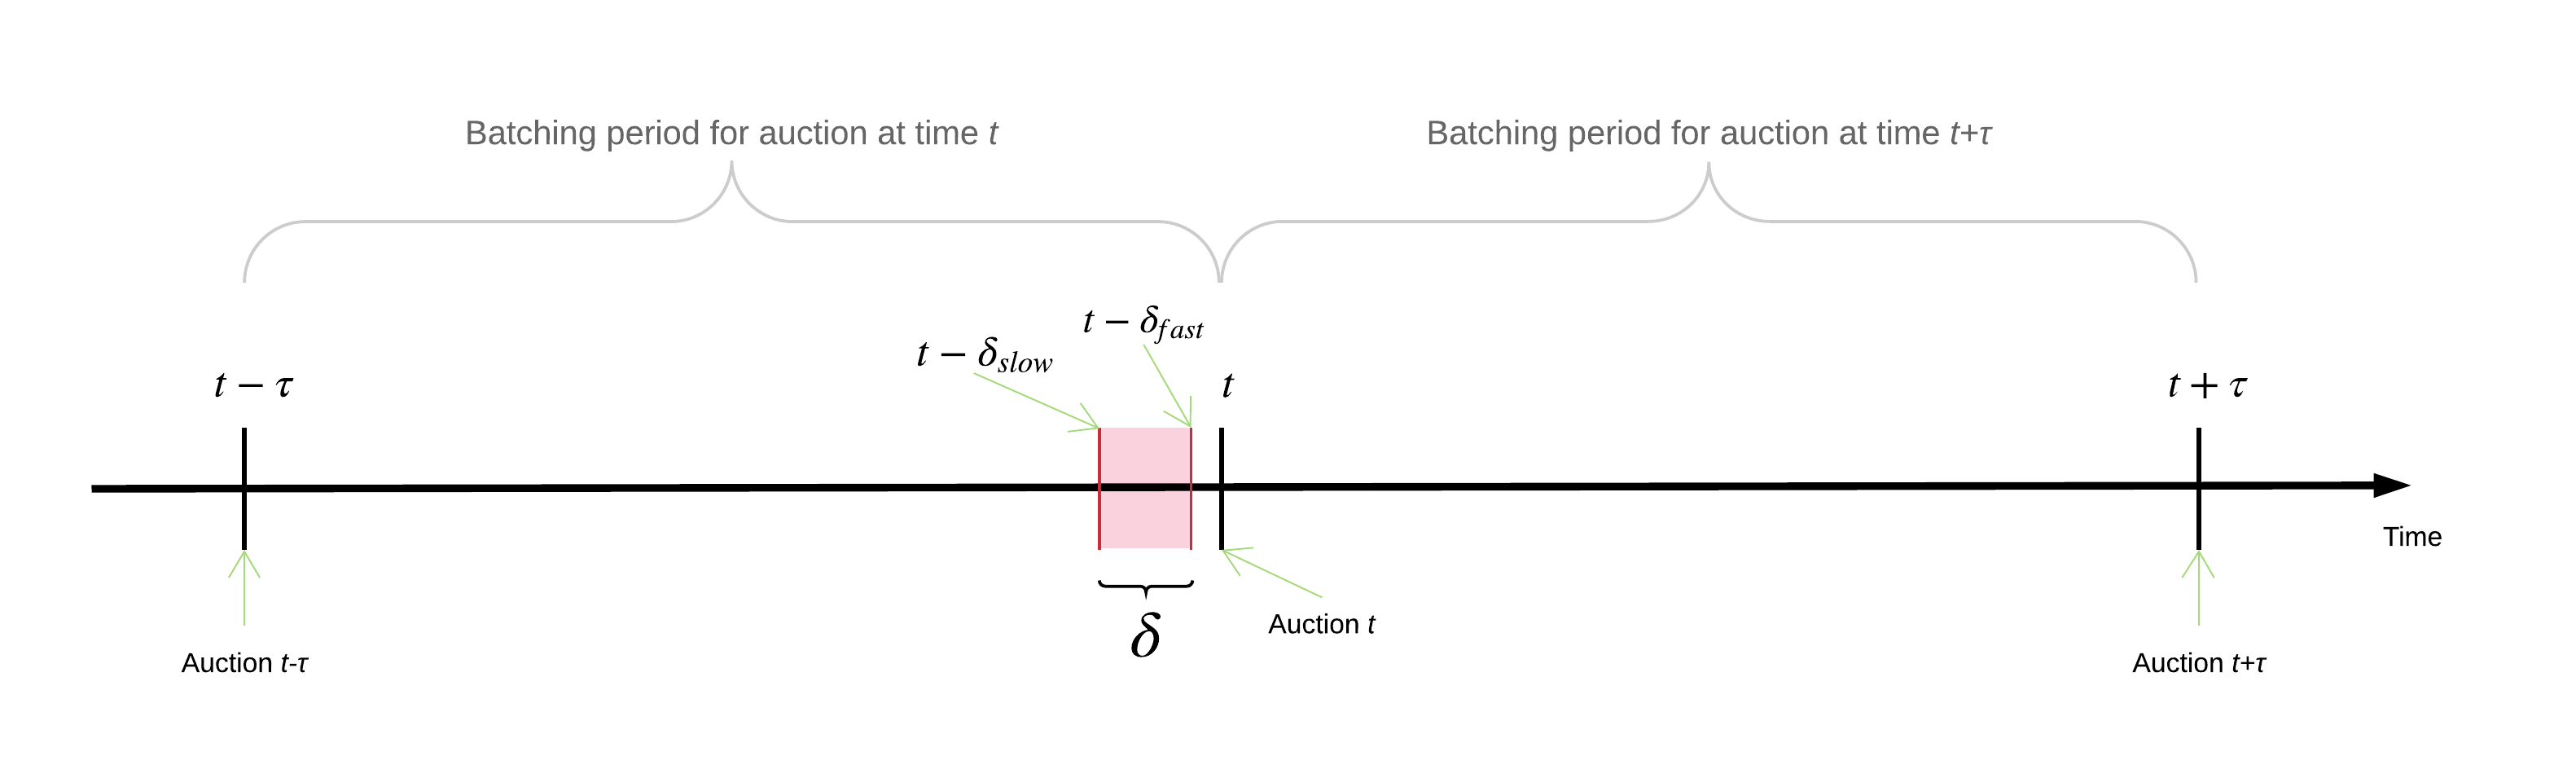
\includegraphics[width=\textwidth]{img/timing_FBA.png}
\caption{\label{fig:FBAtiming}Timing in the FBA format (adapted from \cite{Budish2015}).}
\label{fig:fbaDiagram}
\end{figure}

Under certain conditions, the BCS equilibrium for FBA consists of all traders choosing to act as market makers with zero spread and none of them purchasing fast communication technology. Specifically, \cite{Budish2015} show that if:
\begin{align} \label{eq:BCSFBA}
  \frac{\delta}{\tau} \cdot \lambda_V E\left[J | J>0\right] < c_s
\end{align}
there is no incentive for traders to take the role of a fast sniper in the FBA. Intuitively, the left-hand-side of Equation \eqref{eq:BCSFBA} is the profit attributed to a fast sniper who successfully exploits a unit share posted by a slow market maker when a jump occurs in the interval $\delta$: $\frac{\delta}{\tau} \cdot \lambda_V$ represents the probability of a value jump in the short interval $\delta$ and $E\left[J | J>0\right]$ represents the magnitude of the gain (when $s^*=0$). Since there are no fast snipers in the market, the need for high-speed communication technology vanishes.  Competition focuses purely among makers on price (à la Bertrand) and dictates that all market makers undercut each other until $s^* = 0$ (all bids and offers are set to equal the observed fundamental value, $V$). 

It is important to note that, as in the CDA, makers earn profits in the FBA by transacting with investors. However, since investors submit the best bids and offers within a batching period, the FBA auction often pairs their orders together as transactions. As a result, makers only transact with investors when the number of buying investors within a batch differs from the number of selling investors. Such transactions occur at the market clearing price, $p^*$, which is weakly lower (higher) than  the best bid (offer). Thus, for a given set of player strategies in the market, there are two reinforcing channels by which makers earn lower transaction profits in the FBA relative to the CDA: (1) fewer investor transactions and (2) transactions prices that are closer to the fundamental value of the asset. This reduction in profits is partially offset by smaller losses to sniping.\footnote{Similar to the CDA case, there is the possibility of cooperative equilibria in the FBA. In the Appendix \ref{sec:collusiveEq}, we argue that collusive play is unlikely due to the number or players in each market.}

\subsection{Architecture}

The experimental architecture consists of two components: (1) a laboratory software interface that implements the BCS model and which is specific to each of the market formats (CDA and FBA) and (2) a remote exchange that is specific to each of the formats.

The laboratory software is a high-level computer interface that allows human subjects to continuously tune algorithmic trading strategies during a trading session. As market conditions evolve, these algorithms interact with the remote exchange server at millisecond time granularity. 

Communication latency and the speed with which traders realize their strategies is a central feature of the BCS equilibrium. However, these latencies are technological constraints not related to human physiological limitations. Consequently, in our experiment, the speed at which subjects trade should not depend on their human-reaction time, but solely on the instructions they provide to their algorithms and whether or not they use a costly technology that reduces messaging latency between their algorithms and the exchange.

\subsubsection{Laboratory Interface}
The laboratory component of the architecture is implemented using the Redwood 2 platform. Redwood 2 is a Django-based experiment platform designed for games in continuous time.\footnote{To our knowledge, Redwood 2 the only open-source, browser-based experimental platform that can support all three: continuous-time games, arbitrary graphical interfaces and connection to external market engines as required by our architecture (\url{https://github.com/RedwoodAdmin/RedwoodFramework}).}  The laboratory layer is comprised of the following modules: 
\begin{enumerate}
\item A graphical user interface that displays payoffs, recent history and current state of the market, and trader controls.
\item Individual algorithms (one per subject) that keep track of subjects' choice states and implement their strategies by automatically sending messages to the remote exchange (using Nasdaq's OUCH 4.2 protocol) as market conditions change.
\item A market manager that handles OUCH messages composed by subjects' algorithms and passes them on to the remote exchange. In return, the market manager receives confirmation messages from the exchange, which are forwarded to individual algorithms. The market manager also implements value jumps and investor arrivals from prespecified draws of the Poisson processes describe above.
\end{enumerate}

The user interface for the CDA format is shown in panel (a) of Figure~\ref{fig:UI-CDA}. The \textit{info box} (top) displays basic information about the market state such as the current bid-offer spread, the number of active traders and the cost of speed $c_s$. Traders use the \textit{choice box} (bottom right) to adjust choices at any moment during the trading period. To (re)enter as a market maker, a subject clicks the “Maker” button, or selects a spread ($s_i$) by clicking in the white area of the \textit{choice box}. To (re)enter as a sniper, a subject clicks the “Snipe” button. By clicking the “Out” button, a subject cancels any limit orders, deactivates any algorithms trading on her behalf, and unsubscribes from speed services. The \textit{profit box} (bottom left) displays subjects’ accumulated profit at each moment of time. A subject’s profit jumps if there is an investor arrival that executes against her buy or sell orders, if she snipes, or if she gets sniped. 

\begin{figure}
\centering
(a) CDA \\
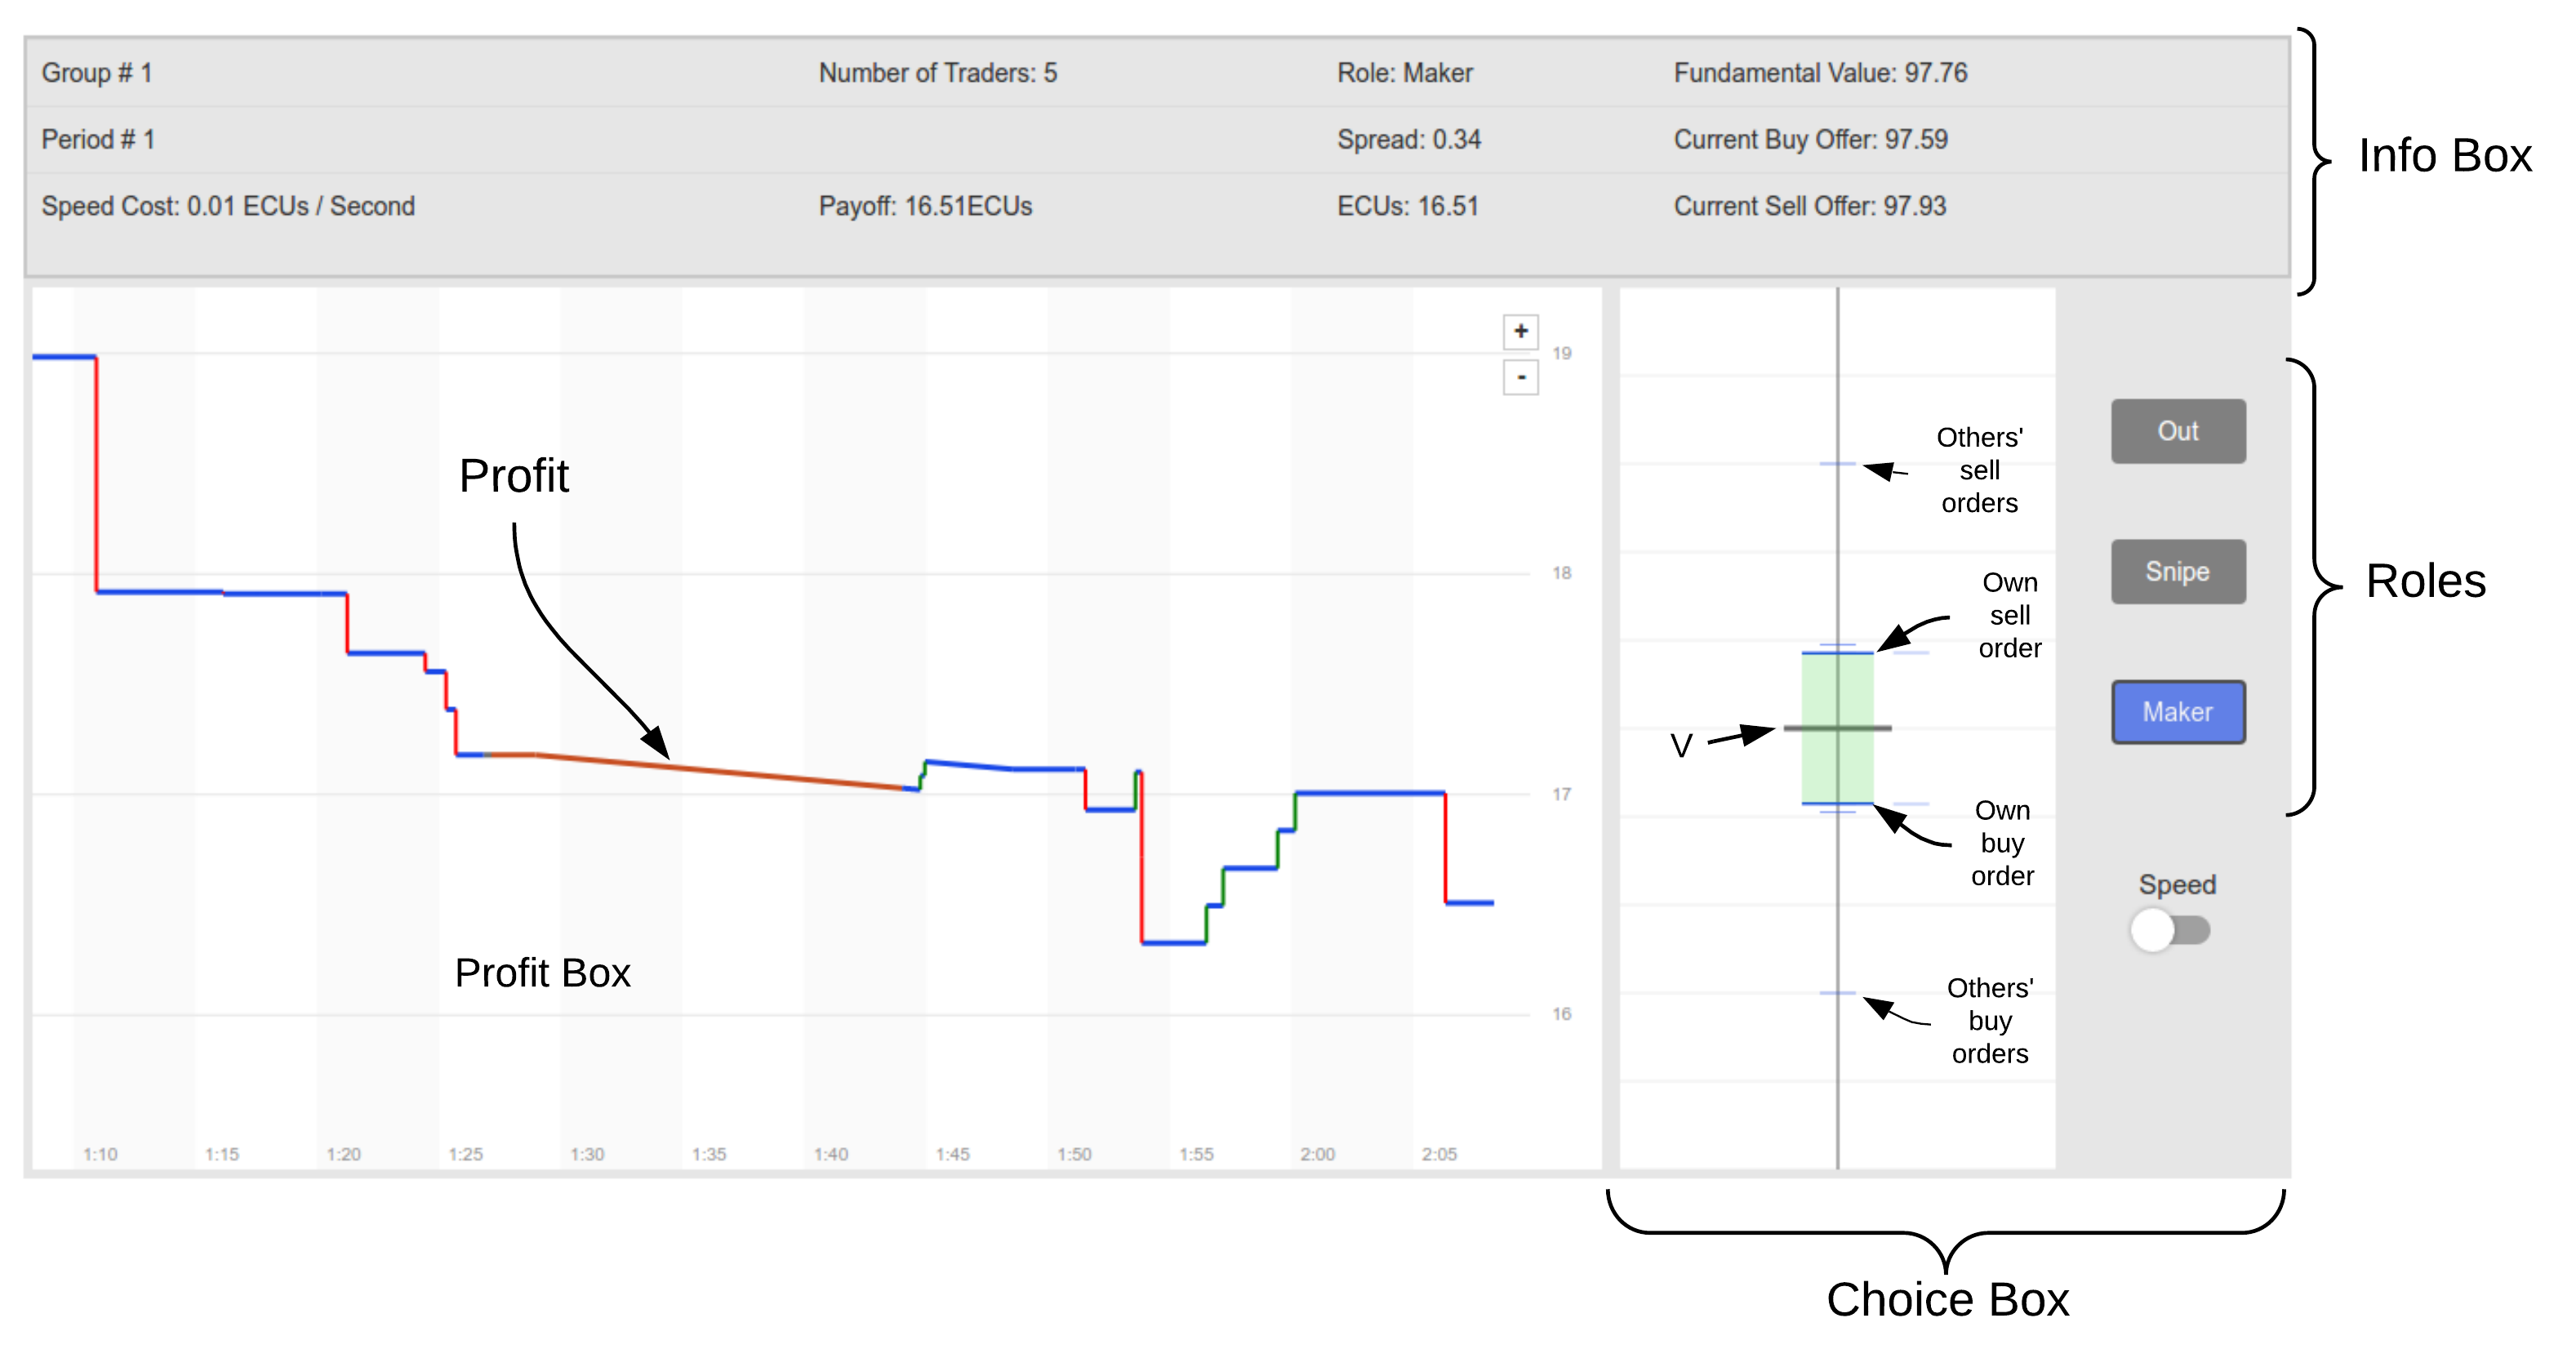
\includegraphics[width=0.95\textwidth]{img/UI-CDA_with_labels.png} \\
(b) FBA \\
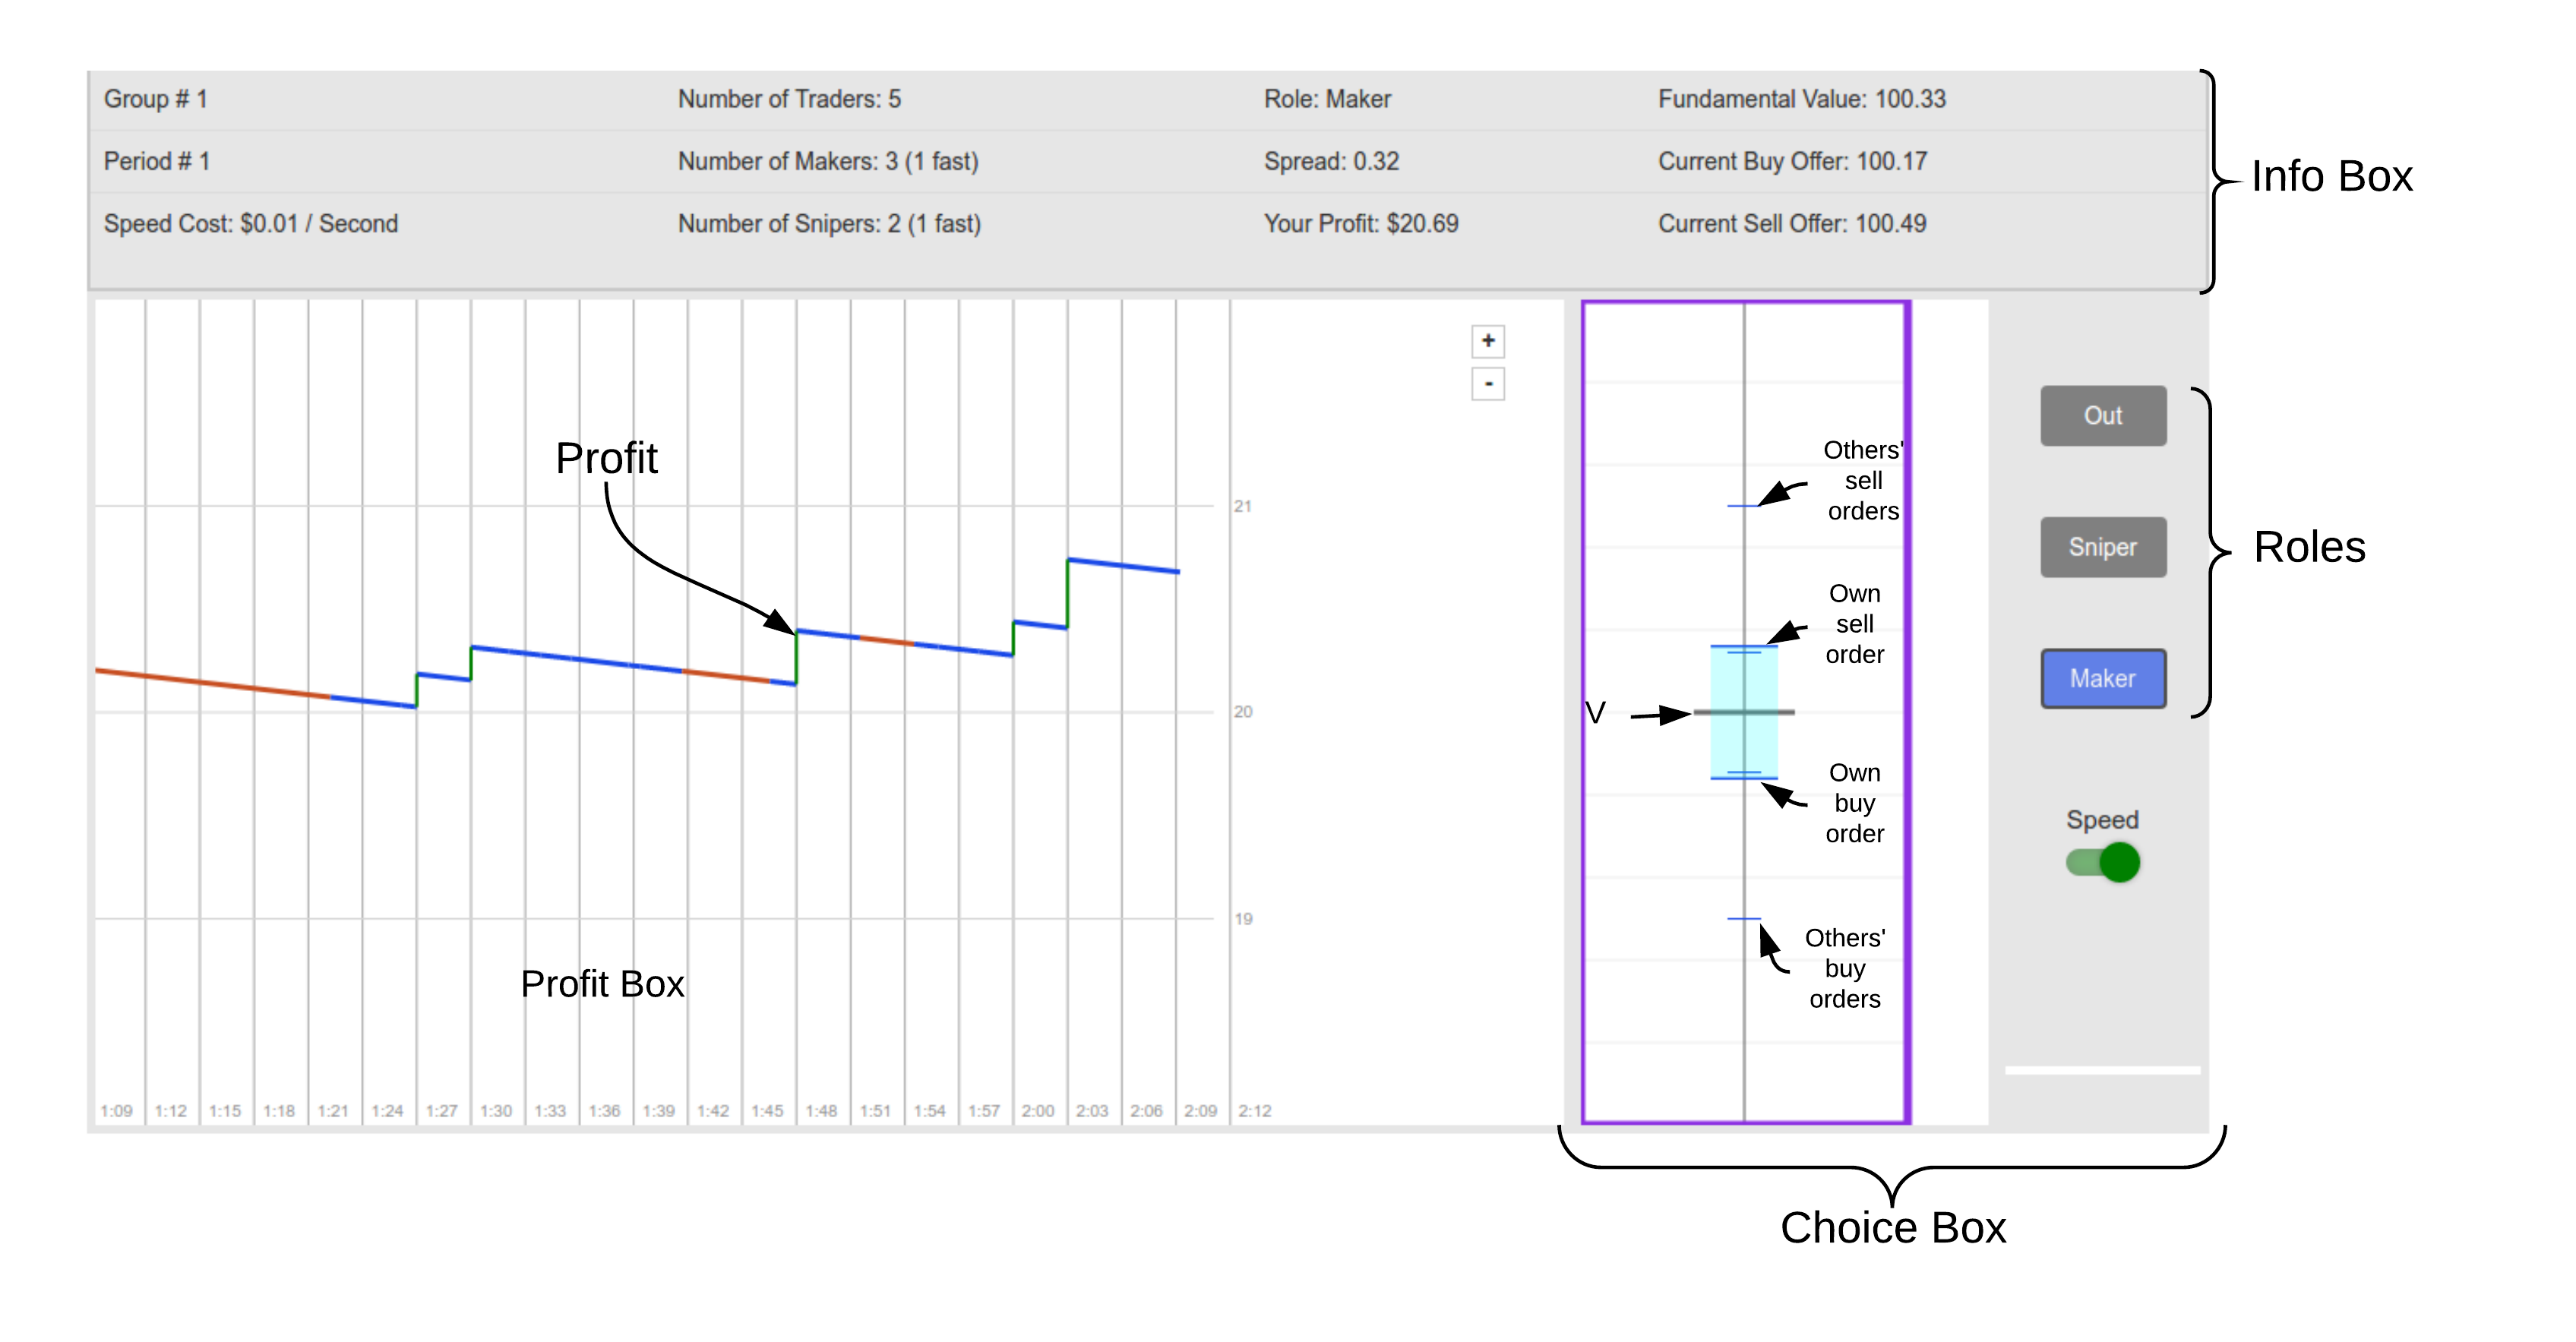
\includegraphics[width=\textwidth]{img/UI-FBA.png}
\caption{Experimental user interfaces for CDA (panel a) and FBA (panel b). \label{fig:UI-CDA}}
\end{figure}

The interface for the FBA format is essentially the same as in the CDA and is shown in panel (b) of Figure~\ref{fig:UI-CDA}.  The FBA choice box includes a time marker that indicates the length and the moment of the auction and the profit box includes markers that indicate the instant of each auction. In addition, the FBA info box displays aggregated information on the roles and speed choices of other traders in the market. This difference from the CDA info box was a programming oversight (they were intended to be identical), but does not constitute a large discrepancy as the information is directly (in the case of number of makers) or indirectly (number of snipers and speed choices) observable from the choice and profit boxes. Further, the interim summary screens in both formats provided the same aggregated information between each four-minute trading period. 

\subsubsection{Remote Exchange}

Each of the market formats we study utilizes a general purpose market engine that acts as a remote exchange. The remote exchanges are patterned after the architecture of exchanges under the Nasdaq OMX umbrella and were developed with the goal of reusing the software infrastructure in future experiments and allowing other researchers the same access.

The remote exchanges are each comprised of two components: a \textit{messaging server} and a \textit{matching engine}. The messaging server follows the Nasdaq OUCH 4.2 specification, which strictly defines a set of incoming and outgoing private messages and their format (the order and byte length of each field within a message). The most common incoming messages (from participant to exchange) sent via OUCH are new order submissions, as well as updates and cancellations of existing orders. Outgoing OUCH messages (from exchange to participants) consist of private confirmations of incoming messages. In addition, the messaging server follows the Nasdaq ITCH 4.1 protocol for public broadcasts of market information. 

The matching engine processes orders relayed from the messaging server, executes transactions according to a specified format (see section \ref{Market Formats}), and reports the results to the messaging server. In both formats we consider, the matching engine maintains a limit order book -- the set of unexecuted, actionable limit orders in the market at a given point in time. Both components are hosted on an Amazon’s Elastic Compute Cloud (EC2) infrastructure located in California, enabling tight control over physical accessibility and communication latencies.\footnote{While there were some alternative options to implement our remote exchange (such as Flex-E-Markets), we opted for developing our own exchange server for two reasons. First, we wanted our platform to be open source so it can be available to other researches for their use and contribution. Second, this exchange was built to exhibit negligible latencies at the messaging and matching engines level. In this way, the laboratory interface can be used to control and implement the menu of different communication technologies (each with its own latency) that is made available to traders.}


\subsection{Treatment Design}
\label{sec:treatments}

A treatment in our experiment consists of a combination of \textit{market format} and a \textit{market configuration}. We study two market formats (CDA and FBA) and three market configurations. In our baseline configuration (C1)  we set $\lambda_I=1/3$, $\lambda_V=1/4$ and $c=0.01$. As argued in Appendix \ref{Calibration}, these values are suggestive of actual dynamics observed in the S\&P 500 exchange traded fund. Substituting these values in the BCS equilibrium Equations (\ref{eq:BCS1}) and (\ref{eq:BCS2}), results in $s^* =  0.324$ and $N^*=5.4$ under CDA. Under FBA, $s^* = 0$ and $N^*=6$, since everyone enters the market in that equilibrium and since there are a total of 6 traders in each market (group). 

For the remaining configurations, we consider variations in the relative jump and investor arrival intensities, as well as the cost of speed, in order to induce larger equilibrium spreads while maintaining the same endogenous population of traders, $N^* \approx 5.4$. In configuration 2 (C2), we use $\lambda_I=1/5$, $\lambda_V=1$ and $c=0.0104$. This could be loosely interpreted as a volatile market, with many asset value changes (once per second) and few investor arrivals. In this case the CDA equilibrium spread is much higher: $s^* = 0.566$. Finally, in configuration 3 (C3) we consider $\lambda_I=1/2$, $\lambda_V=1$ and $c=0.022$, which doubles the cost of speed technology while maintaining the rapidly moving market, but with relatively more investor arrivals. Under this parameterization, the CDA equilibrium spread is $s^* = 0.475$. As with C1, $s^* = 0$ and $N=6$ under FBA for C2 and C3. 
In all configurations, we use a Gaussian jump distribution, $\Delta V(t) \sim \mathcal{N}(0,\sigma=0.5)$,  and the initial value for $V$ is set  at $100$ $ECUs$. Panel (a) of Table \ref{tab:Summary} shows the parameters for each market configuration. Equilibrium predictions for these configuration parameters are shown in Panel (b) of the same table.

In addition to the parameters above, we set $\delta_{slow} = 0.5$ seconds, $\delta_{fast} = 0.1$ seconds for both CDA and FBA in all configurations. We fix the length of a batching period to be $\tau = 3$ seconds, which means that the fraction of time that snipers can exploit slow makers under FBA is $\frac{\delta_{slow}-\delta_{fast}}{\tau} = \frac{0.4}{3} = 0.133$.

We used a between-subjects design to collect data from two sessions for each of the six treatments $\{ CDA, FBA\} \times \{C1,C2,C3\}$. Each session consisted of 12 traders, divided into two independent groups (markets) of six participants and a single treatment was implemented in a session. A session consisted of eight consecutive trading periods of four minutes, with fixed groups across all periods (partner matching). To obtain data for $24$ markets  ($6$ treatments $\times$ 4 groups), we conducted a total of $12$ sessions. Within a trading period, participants were able to change strategies at any moment. However, as highlighted above, the study and architecture were designed to test traders' strategic behavior rather than human reaction times.

Traders were informed in the instructions about the potential size of the market (six traders), latencies ($\delta_{slow}$, $\delta_{fast}$), arrival rates ($\lambda_I$, $\lambda_V$) and  the cost of speed ($c$). 

\subsection{Procedures}

Sessions were conducted at the LEEPS Laboratory of the University of California, Santa Cruz. Recruitment was implemented through LEEPS' ORSEE instance (\url{econlab.ucsc.edu}; \cite{Greiner2015}). Instructions were provided on the computer screen.\footnote{Instructions were extensively discussed and piloted (with students and colleagues) to achieve a balance between clarity and reasonable extension.} After 15 to 20 minutes of reading instructions, a trial round of 90 seconds was launched during which subjects tested the interface with the understanding that it was a trial round -- their actions in that round had no consequences for their earnings and would not comprise part of the formal experiment. Subjects were then given the option to publicly ask questions to the experimenters. The remainder of the session consisted of eight trading periods of four minutes. 
In between trading periods, subjects received a summary screen displaying the distribution and profits of different roles in the corresponding trading period. Each participant received 20 experimental currency units (ECUs) as initial endowment at the beginning of each trading period and final payments were based on the final wealth of a randomly chosen period, using an exchange rate of two ECUs per dollar, plus a \$7 participation fee. The information was provided to subjects in the written instructions. 
%
Although ending a trading period with negative profits was possible (i.e., losing 20 ECUs in the period), this happened only in 1.3\% of the cases and subjects never left the laboratory with less than \$7.
Members of a group (market) were not able to communicate with each other before, during or after the experiment, nor did they learn the identity or characteristics of other participants. Payments were implemented following standard procedures of confidentiality.


\section{Results \label{Results}}

We compare the CDA and FBA market institutions with the following metrics: (1) market liquidity, measured by the fraction of traders who choose to be \textit{market makers}, which is a surrogate for the depth of the order book in this environment; (2) the prevalence of predatory behavior, measured by the fraction of traders who choose to be \textit{snipers}; (3) the penetration of high-speed communication technology in the market, measured by the fraction of traders that choose to subscribe to this service; and (4) transaction costs for investors, measured by the minimum spread among market makers. We also study other auxiliary metrics associated with volatility (e.g.,  the standard deviation of the minimum spread) and informational efficiency (such as the root mean squared deviation between realized prices and fundamental value). Measures of allocative efficiency are less relevant for this paper because we are dealing with a common value asset. 

Prior to reporting our experimental results, several observations are in order. First, one of the CDA sessions (configuration 3) was terminated after 7 (rather than 8) periods because the 1.5-hour session time limit was reached. This affected two of the four markets for that configuration. Second, in certain circumstances, order repricing for market makers resulted in maker-to-maker sniping events. Appendix~\ref{makerSniping} describes these transactions in more detail and shows that they do not affect the BCS equilibrium. We discovered maker-to-maker snipes during initial pilot sessions and decided not to eliminate them, since doing so would violate typical order book rules. However, we did not explicitly acknowledge this feature in the experiment instructions, instead allowing subjects to observe the consequences of these events on their profit and decision screens. Finally, after collecting our experimental data, we discovered that the FBA exchange did not randomize transaction allocation for orders received within the same batch and at the same price. 
Under FBA, time priority should not exist for orders received by the exchange during the same batching period; such priority should only exist for orders received in prior batches and which have not been filled. 
\hl{Although this is a violation of the FBA matching mechanism, this rule change does not have a material impact on market outcomes for the following reasons. First, in the FBA, the protection for market makers from snipers comes mainly from having a batch length substantially larger than the latency differential between fast and slow traders, and not from the random priority of orders at same price within a batch. Second, this rule change affected a very small fraction of orders (only those with identical prices within a single batch) and, at worst, provided an increased incentive to purchase fast communication services (which is not the equilibrium and it is not the prevalent behavior in our experiments).}
Revising the system to allow for randomization of orders during auctions would potentially yield results that are even more congruent with predicted equilibria.

\subsection{Subject Choices}

To quantify treatment effects on choices made by subjects, we estimate the following model: 
\begin{align} \label{eq:RegSpec}
y_{g,t} & = \sum_{j=1}^{3} \left[ \alpha_j Cj_{g,t} + \gamma_j  Cj \times FBA_{g,t}   \right]  + \epsilon_{g,t},
\end{align}
where $y_{g,t} \in \{Maker_{g,t},Sniper_{g,t},Speed_{g,t},MinSpread_{g,t}\}$ is indexed by group and time, $Cj$ is a dummy variable for market configuration $j \in \{1,2,3\}$, and $Cj \times FBA_{g,t}$ is the dummy variable indicating  the interaction between configuration $j$ and the FBA format. 
In this context, since there is no constant in the regression, $\alpha_j$ captures the mean of $y$ in CDA configuration $j$, and $\gamma_j$ captures the FBA - CDA mean difference for $y$ in configuration $j$. 
We estimate this model using a three-second time resolution, excluding the first ten seconds of each period to account for starting effects, and the first two periods of each session to account for possible learning. The estimation was done by combining data for all formats and configurations.  The coefficients are OLS estimates and standard errors are cluster-robust at the group level.  The regression results are reported in Table \ref{tab:Regressions}. 
\begin{table}
\centering
\begin{tabular}{l*{5}{c}}
\toprule
&\multicolumn{1}{c}{(1)}         &\multicolumn{1}{c}{(2)}      &\multicolumn{1}{c}{ (3)}     &\multicolumn{1}{c}{(4)}    &\multicolumn{1}{c}{(5)}         \\
&\multicolumn{1}{c}{Maker (\%)}         &\multicolumn{1}{c}{Sniper (\%)}         &\multicolumn{1}{c}{Speed (\%)}         &\multicolumn{1}{c}{Min. Spread}         &\multicolumn{1}{c}{RMSD}         \\
\midrule
Configuration 1                  &       54.13\sym{***}&       30.89\sym{***}&       56.12\sym{***}&       0.226\sym{***}&       0.347\sym{***}\\
                    &     (1.640)         &     (2.959)         &     (2.972)         &    (0.0438)         &   (0.00474)         \\
[1em]
Configuration 2                  &       30.27\sym{***}&       58.11\sym{***}&       69.20\sym{***}&       0.678\sym{***}&       0.512\sym{***}\\
                    &     (4.507)         &     (3.294)         &     (1.594)         &     (0.114)         &   (0.00918)         \\
[1em]
Configuration 3                  &       40.03\sym{***}&       49.51\sym{***}&       69.02\sym{***}&       0.706\sym{***}&       0.460\sym{***}\\
                    &     (2.368)         &     (2.888)         &     (4.498)         &    (0.0374)         &    (0.0170)         \\
[1em]
FBA $\times$ Config. 1         &       24.88\sym{***}&      -10.95\sym{*}  &      -36.15\sym{***}&      -0.123\sym{**} &      -0.135\sym{***}\\
                    &     (5.022)         &     (5.507)         &     (5.399)         &    (0.0439)         &    (0.0119)         \\
[1em]
FBA $\times$ Config. 2   &       49.08\sym{***}&      -44.23\sym{***}&      -37.82\sym{***}&      -0.502\sym{***}&      -0.102\sym{***}\\
                    &     (6.494)         &     (6.214)         &     (3.968)         &     (0.118)         &    (0.0307)         \\
[1em]
FBA $\times$ Config. 3         &       33.10\sym{***}&      -35.55\sym{***}&      -48.37\sym{***}&      -0.560\sym{***}&     -0.0791\sym{***}\\
                    &     (5.255)         &     (4.309)         &     (5.024)         &    (0.0422)         &    (0.0246)         \\
\midrule
Observations        &       10934         &       10934         &       10934         &       10934         &         142         \\
\bottomrule
\multicolumn{4}{l}{\footnotesize \sym{*} \(p<0.10\), \sym{**} \(p<0.05\), \sym{***} \(p<0.01\)}\\
\end{tabular}
\caption{\label{tab:Regressions} {\small OLS estimates for Equation~\eqref{eq:RegSpec}. The dependent variables in models 1--3 are, respectively, the average percentage of traders choosing to be makers,  snipers, and subscribers to speed services. The dependent variables in models 4 and 5 are, respectively, the average minimum spread and the market-level RMSD. The regressions for all dependent variables except RMSD are conducted with data at the three-second resolution. We exclude the first ten seconds of each period and the first two periods of each session to account for starting effects. Group-level clustered standard errors are reported in parentheses.}}
\end{table}

\subsubsection*{Result 1: More subjects choose to be market makers under FBA.}
Model 1 of Table~\ref{tab:Regressions} shows that the fraction of market makers is between 25\% and 50\% higher under FBA than CDA, with higher values associated with configurations 2 and 3.
Recall that relative to configuration 1, the market under configuration 2 experiences jumps in the fundamental value roughly four times more often, has $40\%$ fewer investors, and has nearly identical cost of speed. Configuration 3, on the other hand, also has four times as many jumps in the fundamental value, but receives 1.5 times the number of investors, and has double the cost of speed. Thus, both configurations 2 and 3 can be regarded as volatile markets, which is costly to market makers, but configuration 3 partly compensates makers with additional income through investors, whereas configuration 2 provides even lower investor income, relative to the baseline calibration. In addition, under configuration 3, all subjects bear a higher cost of speed (makers and snipers). Thus, the results in Table 1 suggest that increased market making under FBA is positively related to volatile environments and fewer investors.

Since market makers are constrained to limit orders of unit size, the fraction of subjects acting as market makers is a direct measure of liquidity or market depth. Hence, the regression results demonstrate that FBA has a positive effect on liquidity that is statistically significant. Moreover, separate tests of the hypotheses $\gamma_2 > \gamma_1$ and  $\gamma_3=\gamma_1$ cannot be rejected at the 1\% level, suggesting the liquidity improving effect of the FBA is highest in the most volatile regime with few investor arrivals.

The first row of plots in Figure~\ref{fig:allPlots} depict time series of the fraction of market makers, averaged across all groups within a given treatment. The faint, solid lines represent average values computed at five-second intervals and bold, solid lines represent exponentially-weighted moving averages with ten-second half lives. 
Dashed lines represent equilibrium values under the BCS model. Each panel of the plot depicts the full time series for a session, concatenating the metrics across the eight four-minute periods, which are visually separated by alternating gray and white vertical bands. To smooth start-up effects within periods, in which players' default state is "Out", we do not include the first ten seconds of each period in the plot.
\begin{figure}
\centering
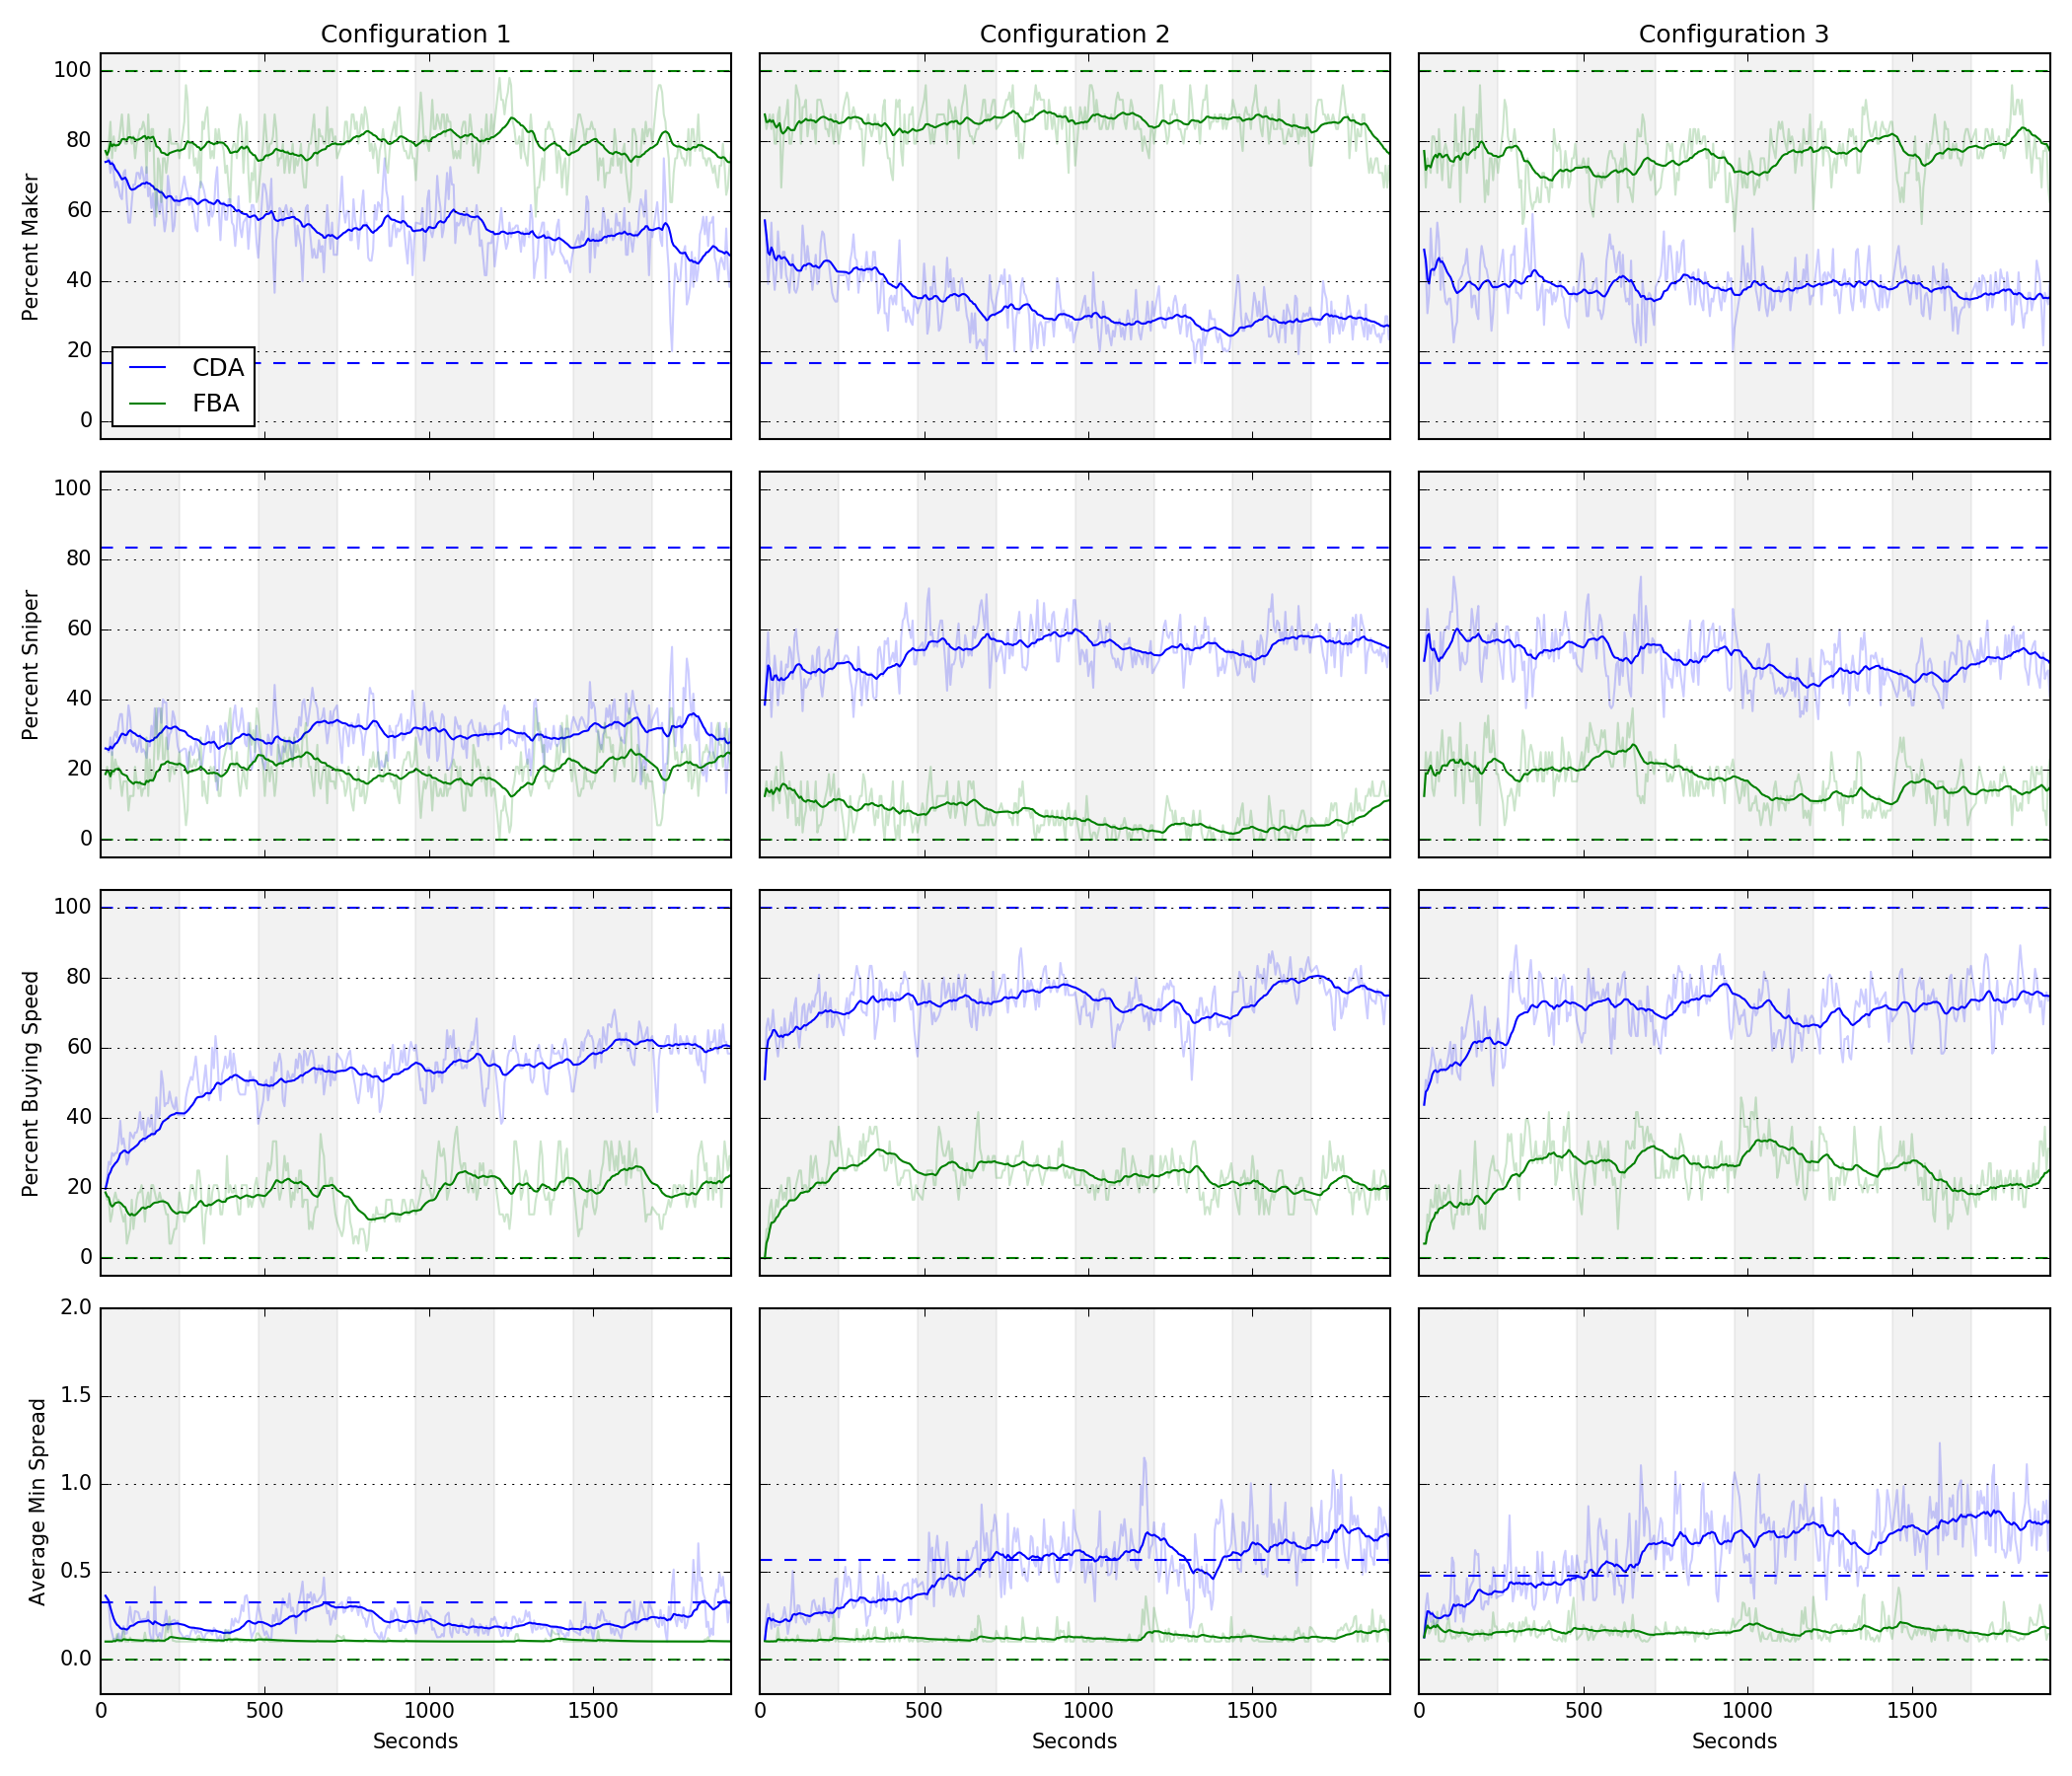
\includegraphics[width=1\textwidth]{img/allPlots.png}
\caption{Time series of subjects' actions: strategies, speed subscriptions and minimum spread. {\small In each box, we plot traders' strategies in CDA (blue lines) and FBA (green lines). Each column of the figure represents a market configuration and each row represents a variable related to the average of the outcome across groups. 
The dashed lines correspond to theoretical equilibrium values predicted by the BCS model. Faint solid lines correspond to observed time series sampled at five-second intervals and bold solid lines are their exponentially-weighted moving averages with a ten-second half life.} \label{fig:allPlots} } 
\end{figure}

The blue lines in Figure~\ref{fig:allPlots} correspond to equilibrium and observed values under CDA and the green lines correspond to those of the FBA. Under BCS, the equilibrium number of makers in the CDA is predicted to be $\frac{1}{N}*100 = 100/6 = 16.67\%$ for all configurations, whereas the the FBA equilibrium is $100\%$ for all configurations.
In magnitude, the fraction of makers fails to achieve the equilibrium values, but the time series show a separation in the direction of the predicted equilibria: for all configurations the fraction of makers is higher under FBA, and the magnitude of the difference is larger under the volatile configurations, 2 and 3. Interestingly, the fraction of FBA market makers is relatively constant across configurations, and the increased difference in market making under those configurations is largely related to a diminished fraction of makers in the CDA. To the extent that the five-second averages exhibit accurate variation in the data, the time series show a clear statistical separation.

% This might be a good spot to note evidence of learning in the time series.
We should note that we find a mild evidence of learning. Our data shows that subjects behavior in the first two periods was shifting (in some variables until the third period) and mostly stabilize after that. See Figure 3 in the paper. This learning behavior is slightly different between formats. In FBA, for example, the average number of role changes in the first two periods is 11.4 and in the rest of the periods goes down 7.33. In the CDA the number of role changes is higher (consistent with the coordination issues of the predicted equilibrium) and stable in all periods. The prevalence of market making, on the other hand, is declining in the first periods of CDA markets but stable along the whole session in the FBA markets. 

\subsubsection*{Result 2: Fewer subjects choose to be snipers under FBA.}
Predatory behavior (the fraction of traders acting as snipers), reported in model 2 of Table~\ref{tab:Regressions}, is substantially lower for all FBA configurations relative to the CDA, with the difference falling in the range $[10\%,44\%]$.
Notably, the total population of snipers is much higher in the CDA for the volatile configurations (C2 and C3) , and lower in the FBA for those same configurations.
Again, tests of the hypotheses $\gamma_2 > \gamma_1$ and  $\gamma_3=\gamma_1$ cannot be rejected at the 1\% level, suggesting that the FBA has a greater impact on discouraging sniping in the most volatile regime with few investors.

The BCS model predicts the equilibrium percentage of snipers to be $\frac{5}{N}*100 = 500/6 = 83.33\%$ under CDA and $0\%$ under FBA, for all configurations. These values are depicted as blue and green (respectively) dashed lines in the second row of plots in Figure~\ref{fig:allPlots}. As with the percentage of market making, the time series in those plots do not achieve the equilibrium values, but exhibit a clear separation in the direction of the equilibria, with only marginal separation for configuration 1. Again, similar to the percentage of market makers, the difference in the FBA - CDA percentages of snipers is larger in volatile environments with fewer investors.

\subsubsection*{Result 3: Fewer subjects purchase speed under FBA.}
Model 3 of Table~\ref{tab:Regressions} shows that purchases of speed services are consistently lower under FBA. Specifically, the total fraction of traders purchasing speed services under CDA falls in the range $[56\%,69\%]$, while the FBA - CDA differences are in the range $[-48\%, -36\%]$. Equilibrium predictions, that $\alpha_j=100$ and $\gamma_j=-100$ for $j\in\{1,2,3\}$, are rejected at the 1\% level.

The BCS model predicts the equilibrium percentage of players purchasing speed services to be $100\%$ under CDA and $0\%$ under FBA, for all configurations. These values are depicted as blue and green (respectively) dashed lines in the third row of plots in Figure~\ref{fig:allPlots}. Similar to the metrics discussed above, the time series in those plots do not achieve the equilibrium values, but exhibit a clear separation in the direction of the equilibria, and the magnitudes of the differences are slightly larger for configurations 2 and 3.

\subsubsection*{Result 4: Minimum spreads are lower under FBA.}
Transactions costs, measured by the average minimum spread, are predicted by the BCS model to be $s^*=0.324, 0.566$ and $0.475$ for configurations 1, 2 and 3, respectively, in the CDA (see Section~\ref{sec:treatments}) and $s^*=0$ for all configurations in the FBA. Model 4 in Table~\ref{tab:Regressions} shows that observed values are close to the minimum increment of 0.1 ECUs in FBA, while the average CDA spreads are much higher and closer to their theoretical counterparts.\footnote{Our lab interface implemented a minimum spread of 0.1 ECUs.} The FBA - CDA differences in spread were $-0.123$,  $-0.502$, and $-0.560$ ECUs, respectively for C1, C2 and C3, and serve as upper bounds for the differences, since they exclude the many investor-to-investor transactions at the fundamental value (zero spread) that occur in the FBA when an equal number of buy and sell investors arrive within one batch.
In general, these differences closely track equilibrium values: for C2 we do not reject the null hypothesis that $\alpha_1=.566$ and $\gamma_1=-0.46$, while for C1 and C3, the minimum spread values are close to, but statistically distinct from, equilibrium levels.
Despite this, a key comparative static across CDA configurations holds in the data: CDA-C2 and CDA-C3 both have statistically higher minimum spread relative to CDA-C1. 

The BCS equilibrium minimum spreads are depicted as blue (CDA) and green (FBA) dashed lines in the fourth row of plots in Figure~\ref{fig:allPlots}. The observed time series are largely congruent with those values, both in direction and magnitude. Perhaps most interesting is the fact that observed FBA spreads consistently remained at or near the floor of 0.1 ECUs implemented in the lab interface.

Panel (b) of Table~\ref{tab:Summary} reports summary statistics for the metrics outlined above, sampled at one-second intervals, averaged across both time and groups and within treatment. As with Figure~\ref{fig:allPlots}, we exclude the first ten seconds of each four-minute period in order to eliminate start-up effects, and we also exclude the first two periods of each session, to account for learning. Congruent with the results above, those values demonstrate that under the FBA (1) more traders choose to act as makers, (2) fewer choose to act as snipers, (3) fewer choose to purchase speed services, and (4) minimum spreads are smaller.
\begin{table}
\centering
\scalebox{0.9}{
\begin{tabular}{lrcccccc}
\toprule
  & &  \multicolumn{2}{c}{\bf Configuration 1} &  \multicolumn{2}{c}{\bf Configuration 2} 
  &  \multicolumn{2}{c}{\bf Configuration 3} \\
  & & {\bf CDA} & {\bf FBA} & {\bf CDA} & {\bf FBA} & {\bf CDA} & {\bf FBA} \\
\midrule
\multicolumn{8}{l}{{\bf (a) Market conditions}} \\
\midrule
$\lambda_I$  			& &  \multicolumn{2}{c}{1/3} &  \multicolumn{2}{c}{1/5} &  \multicolumn{2}{c}{1/2} \\
$\lambda_V$  			& &  \multicolumn{2}{c}{1/4} &  \multicolumn{2}{c}{1} &  \multicolumn{2}{c}{1} \\
$c_{speed}$  		& &  \multicolumn{2}{c}{0.01} &  \multicolumn{2}{c}{0.01} &  \multicolumn{2}{c}{0.022} \\
\midrule
\multicolumn{8}{l}{{\bf (b) Choices}} \\
\midrule
\multirow{ 2}{*}{Making (\%) } 
					 & Experiment  & 54    & 78.1  & 30.2    & 78.8  & 40.1    & 72.9 \\
                     & Equilibrium & 16.7    & 100 & 16.7    & 100 & 16.7    & 100 \\
                     [0.5em]
\multirow{ 2}{*}{Sniping (\%) } 
                     & Experiment  & 31    & 20.8  & 58.1    & 14.5  & 49.5    & 14 \\
                     &  Equilibrium & 83.3    & 0   & 83.3    & 0  & 83.3    & 0   \\
                     [0.5em]
\multirow{ 2}{*}{Speed (\%) } 
                     &  Experiment & 56.1    & 19.7  & 69    & 31.7  & 69.2    & 20.7 \\
                     & Equilibrium & 100   & 0  & 100   & 0   & 100  & 0   \\
                     [0.5em]
\multirow{ 2}{*}{Min. Spread} 
                     &  Experiment & 0.226    & 0.103  & 0.677    & 0.179  & 0.709    & 0.147  \\
                     & Equilibrium & 0.324    & 0 & 0.566    & 0  & 0.475    & 0  \\
\midrule
\multicolumn{8}{l}{{\bf (c) Market stats}} \\
\midrule
\multirow{ 2}{*}{ $Std(P_t-P_{t-1})$  }
						&  Experiment & 2.51 & 0.561 & 4.62 & 1.00  & 6.68 & 1.11 \\
                     & Equilibrium & 0.241    & 0.289 & 0.276    & 0.327  & 0.235    & 0.430  \\
                     [0.5em]
\multirow{ 2}{*}{$Std(MinSpread)$  }
						&  Experiment & 0.204 & 0.0235 & 0.536 & 0.144 & 0.394 & 0.127 \\
                     & Equilibrium & 0    & 0 & 0    & 0  & 0    & 0  \\
                     [0.5em]
\multirow{ 2}{*}{Status Changes  }
						& Experiment & 20.5 & 6.26 & 31.6 & 6.26 & 17.0 & 7.34 \\
                     & Equilibrium & N/A   & 0 & N/A    & 0  & N/A    & 0  \\
                     [0.5em]
\multirow{ 2}{*}{$RMSD(P_t-V_t)$ } 
						&  Experiment  & 0.347 & 0.212 & 0.512 & 0.410 & 0.460 & 0.381 \\
                     & Equilibrium & 0.223    & 0.136 & 0.329    & 0.211  & 0.372    & 0.276  \\
                     [0.5em]
\multirow{ 2}{*}{\# Transactions}                         
  					 & Experiment & 156 & 85.2 & 172 & 99.3 & 248 & 134 \\
  					 & Equilibrium & 106 & 80 & 100 & 48 & 147 & 120 \\
                     [0.5em]
\multirow{ 2}{*}{Period Profits} 
                     & Experiment  & .0869 & .435 & .603 & .372 & 4.31 &  1.52 \\
                     & Equilibrium & 0    & 0 & 0    & 0  & 0    & 0  \\
\bottomrule
\end{tabular}
}
\caption{Summary statistics for experimental data. \small Panel (a) Shows the parameters of the three configurations we use in the experiments. Panel (b) reports the average percentage of subjects acting as market makers, snipers, average percentage of subjects purchasing speed services, and the average minimum spread posted by market makers. Values are sampled at three-second intervals and averaged across time and subjects within each treatment. Predicted equilibrium values are reported below observed averages. Panel (c) reports summary measures related to volatility (standard deviation of price changes and minimum spread, number of strategy/role changes), informational efficiency (root mean squared deviation from price to fundamental value),  volume (number of transactions), and profits. For both panels, we exclude the first ten seconds of each period and the first two periods of each session to account for starting effects. \label{tab:Summary}}
\end{table}

% collusive play.
Although BCS discussed equilibrium for this repeated games is based on the "naive" extension of the static Nash equilibrium at each instant (stage) for the CDA (FBA), there is the possibility of collusive behavior in our experimental markets. 
In Appendix \ref{sec:collusiveEq} we discuss the form collusive play would take and the relevant literature. Our data indicates, however, that that human trades in both market formats exhibited behavior more congruent with competitive, rather than collusive, play. Collusive play in these undercutting games (both CDA and FBA) would imply prevalence of market making at maximum spreads and no purchase of speed. 
Instead we observe that most markets operated closer to competitive play: market spreads were always around the competitive equilibrium predictions far away from collusive behavior prediction. 
In the case of the FBA, the market spread was almost every time against the lower bound of the admissible spread in the computer interface. 
In the case of CDA, although market making was significantly more common than the static Nash equilibrium prediction, majority of traders subscribed to speed and, again, spreads were around the competitive equilibrium, far away from collusive play (see Appendix \ref{sec:collusiveEq} for further discussion). 
All this is consistent with the theoretical insight and empirical findings of existing literature suggesting that cooperation is rarely observed when the game has three or more players.


\subsection{Market Statistics}
\label{marketStatsSection}

Panel (c) of Table~\ref{tab:Summary} reports summary statistics that measure volatility of prices, volatility of strategy choices (changes of roles), pricing deviations from fundamental value, number of transactions, and trader profits. The first two rows of panel (c) provide a measure of transaction price volatility via the standard deviation of transaction price differences, $Std(P_t-P_{t-1})$. We derive the equilibrium equations that govern these values under CDA and FBA in Propositions~\ref{stdDeltaPCDA} and \ref{stdDeltaPFBA}, and report those values for each experimental configuration in the second row of panel (c). The equilibrium CDA values are quite constant across configurations, ranging from 0.241 to 0.276 ECUs. The FBA values are all larger, primarily due to the fact that they measure volatility over 3-second time (batch) intervals, and they are substantially larger for the more volatile configurations, ranging from 0.289 to 0.430 ECUs. The data, on the other hand, show that observed price differences under FBA are roughly two or three times more volatile than their theoretical counterparts, and are between five and 7.5 times more volatile in the CDA configurations, with price volatility higher (for both CDA and FBA) in configurations 2 and 3.

Rows 3-6 of panel (c) report volatility measures related to traders' choices: the standard deviation of the minimum spread and the average number of changes in trading strategy (status) by subjects within a trading period. In equilibrium, the standard deviation of minimum spread should be zero since makers always choose the fixed equilibrium spread, $s^*$. In the data, the standard deviation of minimum spread is nonzero but very low under FBA, and between three and five times greater under CDA, with higher values under configurations 2 and 3.
The model, however, makes no theoretical statement about frequency of strategy switching in the CDA since it only demands a fixed strategy profile in aggregate, while under the FBA there should be no switching since all traders play an identical strategy. Empirically, status changes are between two and 3.5 times greater under the CDA configurations, relative to FBA. The coordination difficulties that can only arise in the CDA are compatible with the CDA exhibiting a higher number of strategy changes than the FBA.

Rows 7 and 8 of panel (c) report the root mean squared deviation (RMSD\footnote{\label{footnoteRMSD} $RMSD = \sqrt[]{\frac{\sum(P_t-V_t)^2}{N_{trans}}}$, where $N_{trans}$ represents the number of transactions within a trading period.}) of transaction prices relative to the contemporaneous fundamental value. We derive the equilibrium equations that govern these values under CDA and FBA in Propositions~\ref{rmsdCDA} and \ref{rmsdFBA}, and report those values for each experimental configuration in the eighth row of panel (c). The theoretical CDA values range from 0.223 to 0.372 ECUs, while the FBA values are between 1.3 and 1.6 times smaller, ranging between 0.136 and 0.276 ECUs. Empirically, the RMSDs are between 1.2 and 1.9 times larger than their theoretical counterparts, with the CDA values consistently larger than those under FBA.

To additionally measure the effect of treatments on RMSD, Model 5 of Table~\ref{tab:Regressions} reports the following regression:
\begin{align} \label{eq:RegSpecRMSD}
RMSD_h & = \sum_{j=1}^{3} \left[ \alpha_j Cj_{h} + \gamma_j  Cj_{h} \times FBA_{h}   \right]  + \epsilon_{h}.
\end{align}
The regression is fit at the level of trading period and group ($h$), and therefore utilizes 142 observations.\footnote{Six treatments with four groups each, trading in periods 3-8, less two group-periods because of the session that stopped after period seven.} 
Consistent with the equilibrium predictions outlined in above, RMSD is lower under FBA. Specifically, RMSD under CDA is in the range $[0.347,0.512]$, while the FBA - CDA differences are in the range $[-0.135, -0.0791]$. 

Rows 9 and 10 of panel (c) report the number of transactions and trading profits earned by makers and snipers during the experiment. In equilibrium, the number of CDA transactions should be
\begin{align}
\label{eq:CDA_trans}
N_{trans} & = 240 \lambda_I +  240 \lambda_V \textrm{Pr}\left(J > \frac{s^*}{2}\right) \frac{5}{6},
\end{align}
where 240 is the length of each trading period in seconds. The respective equilibrium values of $N_{trans}$ for configurations 1, 2 and 3 are 106, 100 and 147, which are much lower than the observed values reported in row 9 of panel (c). Under the FBA, the number of equilibrium transactions is $240 \lambda_I $, or 80, 48 and 120 for configurations 1, 2 and 3, which, aside from configuration 2, are close to the observed values in row 9 of panel (c). The FBA counts include transactions that occur between investors, and aside from configuration 2, the theoretical values are close to the observed values. 
The discrepancy in C2 emerges from the high frequency of value jumps and  transactions of makers sniping makers, described in Appendix~\ref{makerSniping}.

The last two rows of Table~\ref{tab:Summary} report net profits for makers and snipers in ECUs. Equilibrium profits for both formats are identically zero. Observed values are calculated by summing all gains and losses in each trading period and averaging the aggregated values across periods and subjects (or by subtracting the endowment from the end-of-period profits).  In all configurations, observed profits are positive, ranging from 0.0869 to 4.31 ECUs, with configuration 3 having the highest profits for both CDA and FBA formats. 
For the markets included in this calculation (period > 2), only 0.5\% of the 840 cases (140 markets times six traders) resulted in a trader finishing the period with a negative total profit.

Although the BCS environment is not suited for studying measures of allocative efficiency, such measures are of tangential interest. The percentage of unfilled investor orders is such a measure.  Both formats predict that 100\% of investors orders are filled in equilibrium, while in practice, temporary coordination failure in the CDA (such as all traders acting as snipers) can result in a lower percentage. Indeed, while only 0.14\% of investors' orders were not filled in the FBA, the same value was 2.57\% in the CDA.

It is also important to note that the purchase of speed is a measure of deviation from Pareto efficiency. Since traders improve profits off by collectively abstaining from speed purchases, increased use of fast communication technology is associated with social waste. This is due to the fact that $V(t)$ is publicly observable: in such an environment, faster communication technology serves no purpose in acquiring more or better information. 

In summary, the measures in panel (c) of Table~\ref{tab:Summary} show that the FBA reduces the volatility of transaction prices and minimum spreads, enhances price efficiency, results in more stable trader choices, and is more closely aligned with equilibrium profits.

\subsection{Transitory Market Dynamics}

As in real financial markets, subjects in our experiments observed information regarding the trading environment in real time. This included explicit information on the total number of market makers and their (unattributed) spreads, as well as implicit information on the presence of snipers, the volatility of the asset, and the frequency of investor arrivals. To understand the dynamics of the market and the possible effects of transitory changes in the environment on subjects' decisions, we fit a vector autoregression of the form:
\begin{align}
	\bmath{y}_t & = \bmath{a} + \bmath{\Phi} \bmath{y}_{t-1} + \bmath{\varepsilon}_t \label{eq:var1} \\
    \bmath{y}_t' & = [\%Sniper_t, \%Speed_t, MinSpread_t, Turbulence_t], \label{eq:var2}
\end{align}
where, as before, $\%Sniper_t$ is the average fraction of subjects choosing to be snipers during time interval $t$, $\%Speed_t$ is the average fraction of players choosing to purchase speed services during time interval $t$, and $MinSpread_t$ is the average minimum spread in the market over time interval $t$. $Turbulence_t$ is defined as the ratio of number of price changes to the number of investor arrivals, $\frac{N_{V,t}}{N_{I,t}} $, during time interval $t$ \footnote{We do not include the fraction of market makers in the VAR since it is highly co-linear with the fraction of snipers.}. Since $N_V$ and $N_I$ are exogenously determined by calibrated Poisson processes, we constrain the VAR so that the last element of $\bmath{a}$ and the last row of $\bmath{\Phi}$ are equal to zero, causing the last element of $\bmath{\varepsilon}_t$ to be equal to $Turbulence_t$.
We set the time interval of the regression to be 3 seconds, as this is the natural interval of the FBA treatment (the length of the batch), and is reasonable interval over which to measure transitory effects in the CDA \footnote{We also evaluated the VAR for longer time intervals, with diminishing effects in the interval length, suggesting that subjects' reactions to the changing environment are short term. This is corroborated in the impulse responses that we report below.}.

From the perspective of a market maker, turbulence measures the countervailing forces of price volatility (increased sniping costs) with rate of investor arrivals (increased market making income). Further, the theoretical counterpart $\lambda_V/\lambda_{I}$ plays a direct role in the determination of the BCS equilibrium for the CDA, as seen in Equation~\eqref{eq:BCS1}. Equation~\eqref{eq:BCSFBA} shows that only $\lambda_V$ has an impact on the FBA equilibrium. The constrained VAR in Equations~\eqref{eq:var1} and \eqref{eq:var2} not only allows us to measure the transitory effects of players' choices in one period on subsequent behavior, it also captures the transitory effects of turbulence on each outcome variable, net of related effects on other choices.

Table~\ref{tab:varTable} reports parameter estimates of the constrained VAR(1) for both CDA and FBA. The first row of panel (b) shows that the fraction of snipers, the fraction of subjects purchasing speed and turbulence all have a positive and significant (at least at the 5\% level) relationship with subsequent decisions to snipe. The minimum spread, on the other hand, has a negative relationship, at the 5\% level. 
Interestingly, the only lagged variable to be significantly related to speed purchases, is the fraction of agents purchasing speed, whereas minimum spread is positively and significantly (again, at least at the 5\% level) related to all variables except speed purchases. Panel (b), however shows that the only statistically significant relationships under FBA are variables lagged with themselves. Specifically, turbulence has no impact on subsequent behavior in the FBA. Altogether, the results show that very-short term, innovations in market conditions impact behavior in the CDA, while such effects of transient market changes do not exist in the FBA.

\begin{table}[ht]
\vspace{.1in}
\begin{center}
\begin{tabular}{lccccc}
\hline % ----------------------------------------------------------------
& \multicolumn{5}{c}{{\bf (a)} CDA} \\
\cline{2-6} % ----------------------------------------------------------------
& Constant & $\%Sniper_{t-1}$ & $\%Speed_{t-1}$ & $MinSpread_{t-1}$ & $Turbulence_{t-1}$ \\
\hline % ----------------------------------------------------------------
$\%Sniper_t$ & 10.1\sym{***} & 0.720\sym{***} & 0.0651\sym{**} & -3.14\sym{**} & 0.141\sym{**} \\
& (2.15) & (0.0354) & (0.0320) & (1.24) & (0.0670) \\
$\%Speed_t$ & 10.3\sym{***} & 0.0480  & 0.813\sym{***} & -0.494 & -0.00220 \\
& (1.90) & (0.0313) & (0.0283) & (1.09) & (0.0593) \\
$MinSpread_t$ & -0.00389 & 0.00250\sym{**} & 0.000877 & 0.656\sym{***} & 0.00665\sym{***} \\
& (0.0611) & (0.00101) & (0.000911) & (0.0352) & (0.00191) \\
\hline % ----------------------------------------------------------------
& \multicolumn{5}{c}{{\bf (b)} FBA} \\
\cline{2-6} % ----------------------------------------------------------------
& Constant & $\%Sniper_{t-1}$ & $\%Speed_{t-1}$ & $MinSpread_{t-1}$ & $Turbulence_{t-1}$ \\
\hline % ----------------------------------------------------------------
$\%Sniper_t$ & 4.66\sym{***} & 0.752\sym{***} & 0.0347 & -10.1\sym{**} & -0.0442 \\
& (1.03) & (0.0317) & (0.0331) & (4.13) & (0.0529) \\
$\%Speed_t$ & 5.73\sym{***} & -0.0129 & 0.752\sym{***} & 2.98 & 0.0182 \\
&  (0.995) & (0.0305) & (0.0319) & (3.97) & (0.0509)\\
$MinSpread_t$ & 0.0683\sym{***} & -0.000182 & 0.0000620 & 0.529\sym{***} & -0.000132 \\
& (0.0102) & (0.000313) & (0.000327) & (0.0408) & (0.000523) \\
\hline % ----------------------------------------------------------------
\multicolumn{6}{l}{\footnotesize \sym{*} \(p<0.10\), \sym{**} \(p<0.05\), \sym{***} \(p<0.01\)}\\
\end{tabular}
\end{center}
\caption{Parameter estimates for the constraint VAR(1) in Equations~\eqref{eq:var1} and \eqref{eq:var2}. Standard errors are reported in parentheses. Panel (a) reports CDA estimates and panel (b) reports FBA estimates.}
\label{tab:varTable}
\end{table}

\begin{figure}
\begin{center}
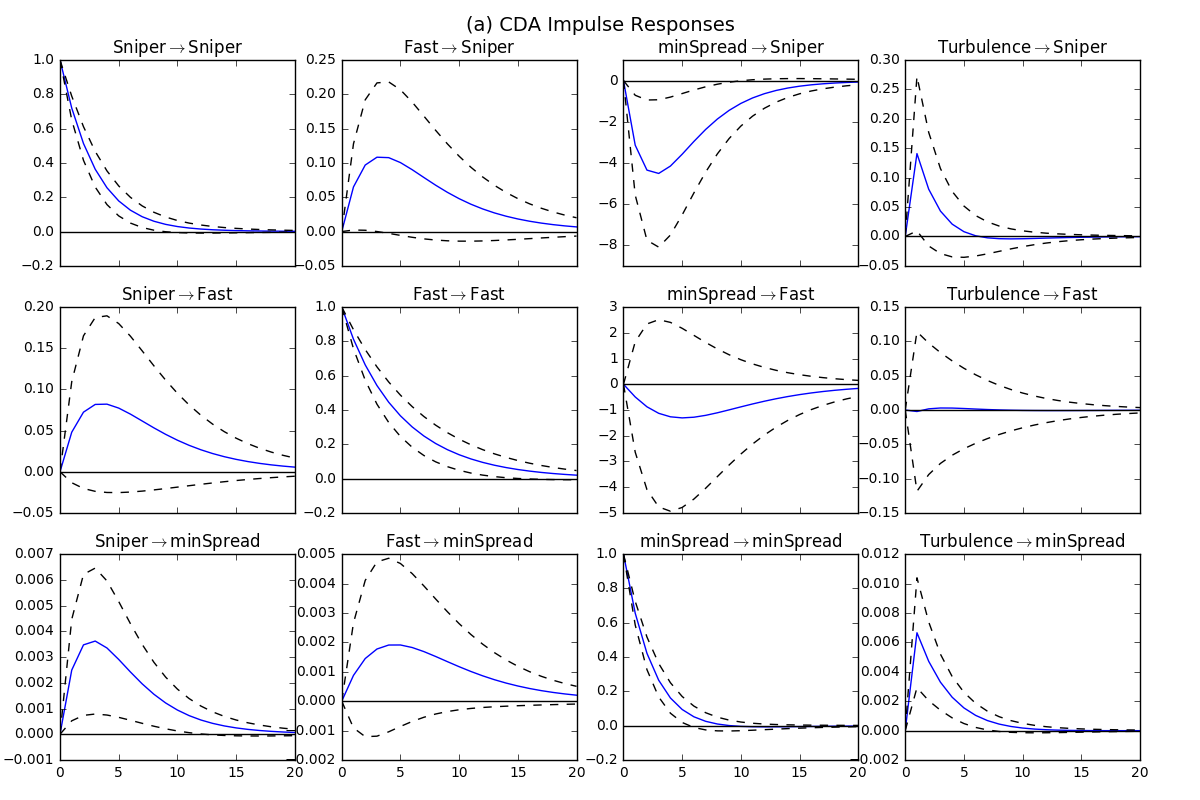
\includegraphics[width=\textwidth]{img/irfCDA.png}
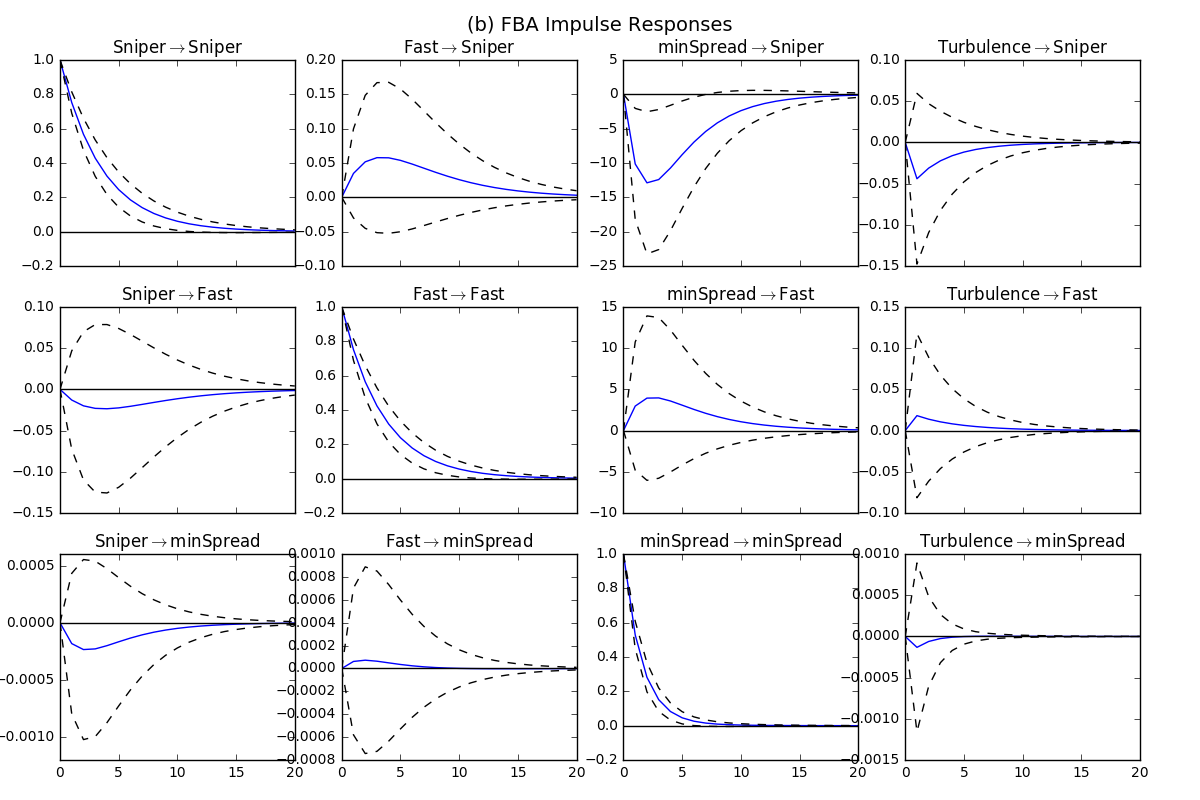
\includegraphics[width=\textwidth]{img/irfFBA.png}
\caption{Unit impulse responses for the estimated VAR under CDA (panel a) and FBA (panel b).}
\label{fig:irfs}
\end{center}
\end{figure}

Figure~\ref{fig:irfs} depicts impulse responses for the estimated VARs reported in Table~\ref{tab:varTable} for a horizon of 20 three-second periods, or 1 minute of clock time. In each case, the impulse responses measure the effect of a one-unit increase in the impulse variable, holding all other variables constant.
The responses in both figures are congruent with the parameter estimates reported in Table~\ref{tab:varTable}. Specifically, under FBA shocks to each of the variables only have autocorrelative effects and no cross-correlative effects in subsequent time periods.
Under CDA (panel (a) of Figure~\ref{fig:irfs}), (1) a transitory 1\% increase in the fraction of snipers leads to a small (no more than 0.003 ECUs), positive and significant increase in the minimum spread for about 40 seconds, (2) a transient 1\% increase in the fraction of subjects purchasing speed services results in an increase in the fraction of snipers by as much as 0.1\% for no more than 10 seconds, (3) a transitory increase in the minimum spread by 1 ECU leads to a significant decline in the fraction of snipers by as much as 4\% for nearly 30 seconds, and (4) a unit increase in turbulence results in a very short (less than 5 seconds), but significant increase in the fraction of snipers and a longer (a little over 20 seconds) and significant increase in the minimum spread, by as much as 0.006 ECUs.

We repeated the VAR analysis using only the final four periods of each session and found that the results were nearly identical to those reported above. This suggests that the short-term dynamics are a permanent feature of the respective formats and not caused by different starting effects or learning patterns. As a whole, our VAR results show that relative to the CDA, the FBA attenuates behavioral responses to short-term shocks in market conditions. We highlight that these are behavioral patterns not predicted by the model, which is silent regarding market dynamics. Understanding this dynamic behavior is an important reason to conduct experiments in the lab and field.

\section{Conclusions \label{Conclusions}}

We use laboratory experiments to empirically study and compare the performance of continuous double auctions and frequent batch auctions as financial market allocation mechanisms. The environment for our experiments follows the model of \cite{Budish2015}, where a single asset is traded on a single exchange and two exogenous processes generate incentives to trade: changes in a publicly-observed fundamental value of an asset and the arrival of market orders from noise traders (\textit{investors}).  In our experiment, human participants (acting as traders) tune algorithms that trade on their behalf. Traders have access to a costly technology that reduces latency of messaging with the (remote) exchange. We emulate modern financial markets by developing an electronic architecture in which information and trading occur at millisecond time granularity and which follows the Nasdaq OUCH messaging protocol. Each of the market formats (CDA and FBA) is studied under three market conditions, varying the degree of volatility in the market and the cost of technology.

We find that, compared to the CDA, the FBA exhibits higher levels of liquidity, less predatory behavior, less investment in communication technology, lower transactions costs, and higher informational efficiency. Specifically, there are between 25-50\% more market markers under the FBA than the CDA, 10-44\% fewer aggressive traders seeking to trade on stale information, and 36-49\% fewer traders purchasing speed technology. 
Further, the average minimum spread among market makers is substantially lower in the FBA, volatility of transactions prices and spreads is lower, and deviations in transactions prices from the underlying asset value are lower as well. As an additional measure of interest, we estimate the sensitivity of traders' behavior to transitory shocks in several market environment variables and find that the sensitivity is statistically absent in the FBA, despite the fact that such shocks have statistically significant short-run effects on behavior in the CDA.

We also find that market behavior is closer to BCS predictions in more turbulent markets. There are two possible explanations for this finding. First, it could be that the mechanisms outlined in \cite{Budish2015} become stronger in stressed markets. Second, markets with greater turbulence might provide more opportunities for learning since information arrives more frequently. Although our evidence suggests that learning cannot explain the finding, our experiment is not designed to discriminate clearly between those two explanations. We leave the study of this question to future research.

Taken together, our results suggest that the frequent batch auction is a welfare improving mechanism for allocating trade within a financial market. Such market designs are of interest to policy makers and regulators, as they reduce both volatility and dead-weight loss, and shift lost surplus to investors with fundamental portfolio needs. Further, our results suggest that exchange operators may find such alternative market designs promising, as they will inherently attract liquidity from fundamental investors and encourage fast traders to forgo expenditure on costly communication technology and instead focus their attention on liquidity provision. 

We recognize that our results are as much a test of the BCS model as a comparison of the FBA and CDA formats, and that they are only relevant to the extent that the model broadly characterizes actual strategies and interactions by agents in the market (which we think it does). Beyond the relatively simple strategy space for agents in this environment, it would be useful to test the robustness of the FBA mechanism to more sophisticated behavior and complex preferences. Such behavior might include traders that place multiple-unit orders (which either deepen liquidity or have substantial price impact), investors that intelligently shred orders through time, and reactive algorithms (for both makers and snipers) that respond to other traders’ strategies rather than to changes in the environment alone. We hope the approach of this paper will generate insights for such research program, and for the development of new theory.

%We believe at least two paths of research will be fruitful in advancing understanding of financial market design: first, studying alternative market formats (e.g, \cite{Kyle2017} and \cite{Aldrich2017}) in comparable laboratory environments, and second, conducting controlled field experiments that exhibit more realistic and complex features. Indeed, within the framework of a larger research project, we intend to implement a public experiment (in the form of a tournament) in which we will study different financial market institutions in a less stylized environment.

%\hl{The coordination involved in the equilibrium of the CDA format in the BCS model and the higher complexity of the corresponding best response function relative to the one in FBA suggest that the degree of sophistication could be more important in the CDA than in the FBA. We leave for future research the theoretical and empirical analysis of the protection that different market formats provide to unsophisticated players.}

%%%%%%%%%%%%%%%%%%%%%%%%%%%%%
%% REFERENCES
\newpage
%\bibliographystyle{plainnat}
\bibliographystyle{asa}
\bibliography{experimentalHFT}



%%%%%%%%%%%%%%%%%%%%%%%%%%%%%
%% APPENDIX 
\newpage
\begin{appendices}
\section{Calibration \label{Calibration}}
\label{sec:calibration}

\cite{Aldrich2017} obtain proprietary data from the IEX exchange for the month of December, 2016. IEX classifies each participant as either an "agency" or "proprietary" trader, the former being the class of traders with a fundamental interest to buy or sell assets (i.e. to maintain an inventory for portfolio reasons). \cite{Aldrich2017} report that IEX agency transactions comprised 10,498,518 shares of the S\&P 500 exchange traded fund (ticker SPY) during the 21 trading days or $21 \times 6.5 \times 60 = 8190$ trading minutes during December, 2016. Since the median trade size is the minimum block of 100 shares, this amounts to $10,498,518/100 \approx 105,000$ total trades during the month, or $105,000/8190 = 12.82$ investor arrivals per minute, or roughly 1 investor arrival every 4.68 seconds. Although IEX represents only a small fraction of equities market share, we believe that most fundamental traders (investors) will utilize IEX in conjunction with other equities exchanges, and hence that their arrival rates would be suggestive of aggregate investor arrival intensities. The result is that in raw time (we discuss time rescaling below), the Poisson intensity parameter for investor arrivals is $\tilde{\lambda}_I = 1/4.68$.

To calibrate $\tilde{\lambda}_V$, the intensity of the Poisson process governing jumps in the fundamental value, we utilize SPY quotation data at Nasdaq, which, given its liquidity and overall market share, is a good surrogate for the SPY national best bid and offer (NBBO). Our sample covers the period 16 June – 11 September, 2014. There are 26,216,524 quotations in the 62-day period, which comprises 1,450,800,000 milliseconds during trading hours, or approximately 1 quote every 55 milliseconds. Defining a jump as any midpoint price change of magnitude at least \$0.01 over the period of four quotations, or 220 milliseconds, resulted in a median of approximately 3978 jumps per day, or one jump every 5.88 seconds (assuming 23,400 seconds during the 6.5 hour equities market trading day). Hence, $\tilde{\lambda}_J = 1/5.88$, prior to time rescaling.

Following \citet{Aldrich2016}, we assume the trade-time distribution of asset price changes, $\Delta V(t)$, is Gaussian with mean zero. Using the SPY data above, we find that $Std(\Delta V(t)) = \$0.007$, or slightly less than the minimum spread of $\$0.01$.  However, given the preponderance of liquidity at SPY best bid and offer and the fact that the minimum spread is set by the SEC, the unconstrained equilibrium spread is widely considered to be less than $\$0.01$. This suggests that the standard deviation of value changes should be of similar magnitude to the equilibrium minimum spread. As the magnitude of the scale parameter is otherwise arbitrary, we set $\Delta V(t) \sim \mathcal{N}(0,\sigma=0.5)$, resulting in a scale parameter that is of the same approximate magnitude as the CDA equilibrium spreads. Further, the choice region for maker spreads in the experiment was set to encompass a region of $4\sigma$ around the fundamental value.

We set $\lambda_V = 1/4$ in our baseline calibration, which leads us to interpret 1 second of lab time as $\lambda_V/\tilde{\lambda}_{V} = 5.88/4 = 1.47$ seconds of raw financial market time. Consequently, we interpret a single four-minute experimental period as approximately $4 \times 1.47 = 5.88$ minutes of financial market time, and the full eight-period session as approximately $8 \times 4 \times 1.47 \approx 47$ minutes of market time. Further, rescaling the investor intensity parameter to experimental time results in $\lambda_I = 1.47/4.68 \approx 1/3$, which is the value of our baseline calibration.

To calibrate the cost of fast communication technology, $c_s$, we use the pricing schedule of McKay Brothers LLC, a premier microwave transmission service. To transmit a single symbol on the long-haul route between the CME data center in Aurora, IL to an equities data center in New Jersey costs \$10,600 per month, or about \$0.02 per second (assuming 22 trading days per month, and 6.5 trading hours per day). Scaling to experimental time, this results in about \$0.015 per second. In our baseline calibration we set $c_s = \$0.01$ per second.

\newpage

\section{Off-Equilibrium Sniping}
\label{makerSniping}

In the BCS equilibrium under CDA, sniping transactions occur between one of the $N-1$ snipers and the single maker. In practice, if there is more than one maker (off-equilibrium) at the time of a jump in the fundamental value, the maker whose orders are repriced first may snipe the maker who is repriced after. These maker-to-maker sniping transactions are not explicitly dealt with in  \cite{Budish2015} and raise the question as to whether they could alter the equilibrium. Empirically, we find the prevalence of these transactions is substantial. However, augmenting the model with this strategy does not extend the set of equilibria, which remains unique up to the aggregate composition of making and sniping strategies.  

We illustrate this type event with an example. Consider a market operating under the CDA. Suppose at $t=0$ the value of the asset is $V=100$ and only two traders are present in the market as makers. Let us refer to these traders as M1 and M2, and assume that they both have a spread of $s=2$ (bids at 99 and offers at 101), and that M1 has purchased speed services (operating at a latency of 100 ms) and M2 has not (operating at a latency of 500 ms). If the value jumps to $V=105$ at $t=700$ ms, M1's algorithm will submit messages to the exchange, updating her bid and offer to 104 and 106, respectively. Those messages will be received at the messaging server at $t=800$ ms and immediately passed to the order book, where M1's new bid of 104 will cross with M2's stale offer of 101. Under typical exchange rules, the order is filled at 101, resulting in a profit (loss) of $105-101 = 4$ to M1 (M2).\footnote{Similar events occur less frequently when makers (fast or slow) are filled by an investor and the asset value changes multiple times during the interval in which new orders are being routed to the exchange. We do not focus on these, as they account for very little total volume.} 

In the equilibrium under FBA, on the other hand, sniping transactions occur between investors and any of the $N$ makers when the value jump occurs too late for makers to update quotes before batch end. In practice, if some makers purchase speed technology (off-equilibrium), maker-to-maker sniping can occur. However, since these events can only happen when jumps occur close to the end of the batch, their prevalence is much less common than in the CDA. Additionally, if one or more traders decide to act as snipers (off-equilibrium), both slow and fast makers will be sniped by investors, fast makers and fast snipers, in that order. As shown below, this is the pattern we find in the data. 

Table~\ref{tab:makerSniper} reports frequency counts of snipes under each of the CDA and FBA configurations. In each case, the number of snipes is decomposed by the roles of the traders participating in the sniping transaction. While the parties of each transaction are clearly defined in the CDA, the same is not true of the FBA: there is no specific attribution of which traders transact with each other in a call-type auction. To make such attributions, we paired sniped traders (those with negative profits) with non-sniped traders in the following priority: (1) fast snipers, (2) fast makers, and (3) investors. Since slow makers and slow snipers never have an opportunity to snipe in the FBA, we make no such attributions. Although our particular attribution order may be somewhat arbitrary, it corresponds to the correct attribution in batches with a single transaction and  the aggregate counts are comparable to those of the CDA.

\begin{table}[ht]
\vspace{.1in}
\begin{center}
\scalebox{0.83}{
\begin{tabular}{l|cc|cc|cc|cc|cc|cc}
\toprule
& \multicolumn{2}{|c|}{Investor} & \multicolumn{2}{c|}{Fast Maker} &  \multicolumn{2}{c|}{Slow Maker} & \multicolumn{2}{c|}{Fast Sniper} & \multicolumn{2}{c|}{Slow Sniper} & \multicolumn{2}{c}{Total} \\
%\midrule
& CDA & FBA & CDA & FBA & CDA & FBA & CDA & FBA & CDA & FBA & CDA & FBA \\
\midrule
\multicolumn{13}{c}{{\bf (a)} Configuration 1} \\
%\midrule
Fast Maker & 32 & 14 & 641 & 10 & 7 & NA & 432 & 0 & 8 & NA & 1,120 & 24 \\
Slow Maker & 22 & 193 & 870 & 112 & 28 & NA & 413 & 55 & 51 & NA & 1,384 & 360 \\ 
\midrule
\multicolumn{13}{c}{{\bf (b)} Configuration 2} \\
%\midrule
Fast Maker & 38 & 49& 397 & 61 & 25 & NA & 1,885 & 0 & 21 & NA & 2,366 & 110 \\
Slow Maker & 29 & 271 & 536 & 639 & 39 & NA & 1,473 & 181 & 83 & NA & 2,160 & 1092 \\
\midrule
\multicolumn{13}{c}{{\bf (c)} Configuration 3} \\
%\midrule
Fast Maker & 135 & 77 & 388 & 31 & 18 & NA & 2,102 & 2 & 23 & NA & 2,666 & 110 \\
Slow Maker &  69 & 448 & 416 & 479 & 22 & NA & 1,048 & 158 & 153 & NA & 1,708 & 1085 \\
\bottomrule
\end{tabular}
}
\end{center}
\caption{Frequency counts of snipes under each of the CDA and FBA configurations, decomposed by the role of the sniper and the trader being sniped.}
\label{tab:makerSniper}
\end{table}

The values in Table~\ref{tab:makerSniper} demonstrate that sniping is much more prevalent under the CDA, with the bulk of CDA snipes done by fast snipers or fast makers.  Interestingly, consistent with the off-equilibrium insight at the beginning of this section, fast makers account for a larger share of sniping in CDA configuration 1, relative to CDA configurations 2 and 3. This latter result is due to the higher population of snipers under the latter two configurations (see Figure~\ref{fig:allPlots} and Table~\ref{tab:Summary}). 
Under FBA, the number of times that fast makers are sniped is about 20 times less than under CDA, and slow makers are sniped roughly 2 to 4 times less. Further, we make the bulk of FBA attributions to fast makers and investors rather than fast snipers.

As successful sniping of any form occurs infrequently under FBA, the consequences of unintentional maker snipes are more important under CDA. That is, makers have access to  similar profit opportunities as snipers, with the additional benefit (cost) of investor transactions (being sniped). We detail the trade-offs to this expanded strategy space below, and prove that the model equilibrium is unchanged. Despite the identical equilibrium, it is possible that the perceived benefit of maker-to-maker snipes may partly explain why our experimental observations are attenuated relative to predicted BCS equilibrium values.

\subsection{Equilibrium with Maker-Snipers in the CDA}
\label{sec:makerSniper}

We now show that extending the BCS model to explicitly account for maker-to-maker sniping leaves the CDA equilibrium intact. 

\begin{proposition} \label{bcsMakerSniping}
Consider an augmented BCS model that allows repriced maker orders to transact with stale limit orders posted by other traders. The equilibrium of the augmented model is identical to that of \citet{Budish2015}.
\end{proposition}

\noindent \emph{Proof} We sketch the proof for the case of the CDA with endogenous entry. Suppose an equilibrium exists with $N$ trading firms acting as market makers, quoting the same spread, $s$, and all purchasing fast communication technology. The profit to each firm would be
\begin{gather}
\lambda_I\cdot\frac{s}{2N} -\lambda_V\cdot\textrm{Pr}\left(J>s\right)\cdot\mathbb{E}\left[J-\frac{s}{2}|J>s\right]\cdot \textrm{Pr}(Sniped) \nonumber \\
\hspace{1.55in} + \lambda_V\cdot \textrm{Pr}\left(J>s\right)\cdot\mathbb{E}\left[J-\frac{s}{2}|J>s\right]\cdot \textrm{Pr}(Sniping) = c_{speed} \label{allMakers1} \\
\Rightarrow \lambda_I\cdot\frac{s}{2N} = c_{speed}. \label{allMakers2}
\end{gather}
The LHS of Equation~\eqref{allMakers1} has positive and negative terms related to sniping which cancel, resulting in Equation~\eqref{allMakers2}. We examine the terms on the LHS of Equation~\eqref{allMakers1} and compare them with the typical profit condition for a maker in the BCS equilibrium (Equation~\ref{eq:CDAmakerProfit}):
\begin{enumerate}
	\item Investor profits under the all-maker equilibrium are shared among all $N$ firms: $\lambda_I \cdot \frac{s}{2N}$. In the BCS equilibrium, a single trading firm acts as market maker and captures all of the profit alone: $\lambda_I \cdot \frac{s}{2
    }$.
    \item Makers can snipe other makers, but it requires a larger jump to do so: the jump must be at least $s$ in magnitude in order for the bid (offer) of a sniping maker to cross with the stale offer (bid) of another maker. In the BCS equilibrium, a jump of magnitude $s/2$ suffices for a sniper to transact with a stale maker quote. In both cases, the sniping profit is $J-\frac{s}{2}$. Thus, the second term on the LHS of Equation~\eqref{allMakers1} breaks down in the following way: (i) $\lambda_V$ is the jump intensity, (ii) $\text{Pr}(J>s)$ is the probability that a jump is big enough for the maker to be sniped, (iii) $\mathbb{E}\left[J-\frac{s}{2}|J>s\right]$ is the expected sniping profit (conditional on sufficiently large jump), and (iv) $\textrm{Pr}(Sniped)$ is the probability that a maker is sniped. The same terms in Equation~\eqref{eq:CDAmakerProfit} are: (i) $\lambda_V$, (ii) $\text{Pr}\left(J>\frac{s}{2}\right)$, which is larger than $\text{Pr}(J>s)$, (iii) $\mathbb{E}\left[J-\frac{s}{2}|J>\frac{s}{2}\right]$, which is less than $\mathbb{E}\left[J-\frac{s}{2}|J>s\right]$, and (iv) $\frac{N-1}{N}$, which is an upper bound for $\textrm{Pr}(Sniped)$ (see below).
\end{enumerate}

Letting $\textrm{Pr}(Sniping)$ denote the probability of a maker successfully sniping another maker, it can be readily shown that the $\textrm{Pr}(Sniping) = \textrm{Pr}(Sniped)$ \citep[e.g. the High School Prom Theorem -- see][]{Davis2009}. Furthermore, these probabilities lie within the open interval $\left(\frac{ \lfloor N/2 \rfloor}{N}, \frac{N-1}{N}\right)$. Thus, the losses attributed to sniping in Equation~\eqref{allMakers1} are exactly offset by the gains, resulting in a cancellation of the second and third terms on the LHS of Equation~\eqref{allMakers1}.

We now explore the profitability of two possible deviations: (1) a single maker quoting a more narrow spread and (2) a single maker switching roles to act as a pure sniper. Maintaining the notation $s^*$ for the BCS equilibrium spread, we let $\hat{s}$ denote the all-maker equilibrium spread. For the first deviation (narrower spread) to be profitable, the following would need to hold
\begin{align}
\lambda_I\cdot\frac{\hat{s}}{2N} & < \lambda_I\cdot\frac{\hat{s}-\varepsilon}{2} \nonumber \\
& \hspace{0.5in} -\lambda_V\cdot\textrm{Pr}\left(J>\frac{\hat{s}+(\hat{s}-\varepsilon)}{2}\right) \nonumber \\
& \hspace{1.3in} \times \mathbb{E}\left[J-\frac{\hat{s}-\varepsilon}{2}|J>\frac{\hat{s}+(\hat{s}-\varepsilon)}{2}\right]\cdot\frac{N-1}{N} \\
& \hspace{0.5in} +\lambda_V\cdot\textrm{Pr}\left(J>\frac{\hat{s}+(\hat{s}-\varepsilon)}{2}\right) \nonumber \\
& \hspace{1.3in} \times \mathbb{E}\left[J-\frac{\hat{s}-\varepsilon}{2}|J>\frac{\hat{s}+(\hat{s}-\varepsilon)}{2}\right]\cdot \textrm{Pr}(Snipe) \label{makerSniper1} \\
\Rightarrow N(\hat{s}-\varepsilon) - \hat{s} & > 2 \cdot \frac{\lambda_V}{\lambda_I} \cdot \textrm{Pr}\left(J>\frac{\hat{s}+(\hat{s}-\varepsilon)}{2}\right) \nonumber \\
& \hspace{1.3in} \times \mathbb{E}\left[J-\frac{\hat{s}-\varepsilon}{2}|J>\frac{\hat{s}+(\hat{s}-\varepsilon)}{2}\right] \cdot (N-1). \label{makerSniper2}
\end{align}
Intuitively, the deviating maker would capture all investor profits at the expense of increased probability, $\frac{N-1}{N} > \textrm{Pr}(Sniped)$, of getting sniped. In Equation~\eqref{makerSniper2}, we have eliminated a positive constant which does not affect the inequality. Taking the limit as $\varepsilon \to 0$, Equation~\eqref{makerSniper2} can be expressed as
\begin{align}
\hat{s} > 2 \cdot \frac{\lambda_V}{\lambda_I} \cdot \textrm{Pr}\left(J>\hat{s}\right)\cdot\mathbb{E}\left[J-\frac{\hat{s}}{2}|J>\hat{s}\right]. \label{deviation1}
\end{align}

Alternatively, if a single maker deviates to act as a sniper, the resulting profit would be
\begin{gather}
\lambda_V\cdot\textrm{Pr}\left(J>\frac{\hat{s}}{2}\right)\cdot\mathbb{E}\left[J-\frac{\hat{s}}{2}|J>\frac{\hat{s}}{2}\right]\cdot\frac{N-1}{N}=c_{speed} \label{sniperDeviation2}
\end{gather}
Thus, a sniper deviation is profitable if
\begin{gather}
\lambda_V\cdot \textrm{Pr}\left(J>\frac{\hat{s}}{2}\right)\cdot\mathbb{E}\left[J-\frac{\hat{s}}{2}|J>\frac{\hat{s}}{2}\right]\cdot\frac{N-1}{N} > \lambda_I\cdot\frac{\hat{s}}{2N} \label{sniperDeviation3} \\
\Rightarrow \hat{s} < 2 \cdot \frac{\lambda_V}{\lambda_I}\cdot\textrm{Pr}\left(J>\frac{\hat{s}}{2}\right)\cdot\mathbb{E}\left[J-\frac{\hat{s}}{2}|J>\frac{\hat{s}}{2}\right]\cdot(N-1). \label{deviation2}
\end{gather}

To determine if a profitable deviation exists, we compare Equations~\eqref{deviation1} and \eqref{deviation2}. If at least one of the conditions is always satisfied, the all-maker equilibrium cannot be supported. This is the case if the RHS of Equation~\eqref{deviation2} is always greater than the RHS of Equation~\eqref{deviation1}:
\begin{equation}
\begin{array}{ccc}
\textrm{Pr}\left(J>\hat{s}\right)\cdot\mathbb{E}\left[J-\frac{\hat{s}}{2}|J>\hat{s}\right]
& < & 
\textrm{Pr}\left(J>\frac{\hat{s}}{2}\right)\cdot\mathbb{E}\left[J-\frac{\hat{s}}{2}|J>\frac{\hat{s}}{2}\right]\cdot(N-1)\\
\\
\Rightarrow \textrm{Pr}(J>\hat{s})\frac{\int_{\hat{s}}(z-\frac{s}{2})2\phi(z)dz}{\textrm{Pr}(J>\hat{s})} 
& < & 
\textrm{Pr}(J>\frac{\hat{s}}{2})\frac{\int_{\frac{\hat{s}}{2}}(z-\frac{s}{2})2\phi(z)dz}{\textrm{Pr}(J>\frac{\hat{s}}{2})}\cdot(N-1)\\
\\
\Rightarrow \int_{\hat{s}}(z-\frac{s}{2})2\phi(z)dz 
& < & 
\int_{\frac{\hat{s}}{2}}(z-\frac{s}{2})2\phi(z)dz\cdot(N-1)\\
\\
\Rightarrow \int_{\hat{s}}(z-\frac{s}{2})2\phi(z)dz 
& < & 
\int_{\frac{\hat{s}}{2}}(z-\frac{s}{2})(N-1)2\phi(z)dz\\
\\
\Rightarrow \int_{\hat{s}}(z-\frac{s}{2})2\phi(z)dz 
& < & 
\int_{\frac{\hat{s}}{2}}^{\hat{s}}(z-\frac{s}{2})(N-1)2\phi(z)dz \\
& & \hspace{1in} +\int_{\hat{s}}(z-\frac{s}{2})(N-1)2\phi(z)dz\\
\\
\Rightarrow 0 
& < & 
\int_{\frac{\hat{s}}{2}}^{\hat{s}}(z-\frac{s}{2})(N-1)2\phi(z)dz \\
& & \hspace{1in} +\int_{\hat{s}}(z-\frac{s}{2})(N-2)2\phi(z)dz. \label{finalCondition}
\end{array}
\end{equation}
Since the RHS of the last equation of System~\eqref{finalCondition} is always positive for $N \geq 3$, we conclude that the all-maker equilibrium cannot be supported. Further deviations can be derived inductively, resulting in the equilibrium as stated in \citet{Budish2015}.

\newpage

\section{Collusive Equilibria}
\label{sec:collusiveEq}

In this section, we address the possibility of collusive behavior in our experimental markets.\footnote{We thank the editor as well as an anonymous referee for suggesting and encouraging us to include this discussion.} In short, our general finding is that human subjects in both market formats exhibited behavior more congruent with competitive, rather than collusive, play. This is consistent with the theoretical insight and empirical findings of existing literature, suggesting that cooperation becomes more difficult when a game has three or more players.
% We discuss the FBA first, since it lies in the more standard paradigm of finitely repeated discrete time games. We do not derive an specific equilibrium prediction but discuss the form such an equilibrium would take if sustainable.
% \subsection{Collusion in finitely repeated discrete-time (FBA)}

In the FBA, which is a repeated game in discrete time, collusive play would imply all traders choosing to be a maker, at positive (arguably maximal) spread, and not buying speed services. Although there is no previous result on collusion that applies directly to this game \citetext{\citealp{Budish2015} focused only on the pure-strategy, instantaneous Nash Equilibrium}, theory and empirical work on Bertrand games and social dilemmas (e.g., prisoner's dilemma) relate to our setting and therefore provide relevant insights.

In Bertrand games, as well as prisoner's dilemma (PD) games, where the Nash Equilibrium is inefficient from the perspective of players, cooperation is not possible if the stage game is repeated a finite number or times. Sub-game perfection implies non-cooperative behavior in the last period and inductively unravels cooperation in all earlier periods. 

However, for the PD, as documented by \citet{Selten1986}, \citet{Friedman2012}, \citet{Embrey2018} and others, unraveling is limited. Indeed when players are able to adjust strategies "quickly" and the game has many periods, cooperation is commonly observed in two-person PD \citep{Friedman2012,Embrey2018}. Departures from non cooperative behavior have been attributed to different underlying features of decision making. As noted in \citet{Embrey2018}, cooperation in a PD stage game is predicted by models where: (1) there is uncertainty about the type and payoffs of other players \citep{Kreps1982}, (2) players generate \textit{epsilon equilibria} \citep{Radner1986,Friedman2012} by optimizing up to an epsilon distance from the maximal payoff, (3) learning is present \citep{Mengel2014}, and (4) traders exhibit limited forward reasoning \citep{Mantovani2016}. Some forms of social preferences could rationalize cooperative behavior as well. 

PD games with $N>2$ tend to display low levels of cooperation \citep[e.g.][]{Barcelo2015}. For $N$-player-, finitely-repeated Bertrand games, empirical and theoretical insights are more sparse. In one shot encounters there is evidence of collusive behavior with two players,  but collusion is infrequently observed when there are three or more players \citep{Dufwenberg2000, Abbink2005, Abbink2008, Orzen2008, Potters2013}. Although there is evidence of some degree of cooperation in repeated two-player Bertrand games \citep[see e.g.][]{Argenton2012}, to the best of our knowledge there are no relevant studies with multiple players, fixed matching, and repetition over many periods. Therefore, the relative contribution of time horizon (in repeated games) and number of participants on cooperative play is an open question. Our experiments indicate that even with hundreds of periods, the number of players would be the prevailing force for shaping (the lack of) cooperation.

The CDA, on the other hand, is a finite-horizon, continuous-time form of an undercutting game. The body of research on undercutting and cooperation games is small, but has relevant insights. Following the work of \citet{Radner1986} and \citet{Simon1989}, \citet{Friedman2012} formalize a model for a continuous-time prisoners dilemma (in addition to a fast-paced, discrete-time PD). They use the notion of epsilon-equilibrium to derive an equilibrium with near-perfect cooperation, where unraveling forces are limited if (1) players are willing to give up a tiny part of their profits and (2) they can react almost immediately. The logic is that the ability to react quickly reduces the risk of loss related to defection and makes a cooperative equilibrium easier to sustain. Their empirical findings are congruent with the existence of a high-cooperation equilibrium in a continuous-time PD. \citet{Park2014} formalizes a similar model where cooperation is sustained on heterogeneous reaction times that are private information. 

Broad theoretical findings for cooperation in continuous-time PD games are, however, ambiguous. Although the literature above predicts full cooperation, a simple extension of a one-shot game predicts that cooperation would not exist, whereas an extended Folk Theorem gives broad predictions with differing degrees of cooperation. Empirically, the experiments of \citet{Horstmann2015} find reduced cooperation in continuous time, in direct contrast to the results of \citet{Friedman2012}. Their work, however, finds that an increase in the number of players substantially reduces cooperation, and is therefore consistent with the findings of the PD and Bertrand literature cited above.

Together, these insights are consistent with our experimental findings: very little cooperation, most likely due to the number of players in each market (six).

\subsection{Predicted Collusive Profits in FBA and CDA}
Collusive behavior in the FBA would result in all traders choosing to be slow makers, quoting the maximal spread, $\bar{S} = 2$. 
%We went ahead and checked what is percentage of time traders were at 90\% or more of fully cooperative behavior.
%We find this occurred a small fraction of the trading time. We also reject the null hypothesis of $s_i=2$ at standard levels of significance. 
%Another way to approach this question is by comparing the observed profits against the collusive levels.
Under these circumstances, expected profits for each player are equal to: 
\begin{align}
\pi_{c}^{FBA} & = \frac{\bar{S}}{N} \cdot T \cdot E [N_I^e],
\end{align}
where $N$ is the number of traders in the market, $T$ is the number of batches (80 per 4-minute trading period),  and $E[N_I^e]$ is the expected absolute difference in the number of buy and sell investors that arrive within a single batch (recall that investors cross with each other before human participants in the FBA). More precisely, $N_I^e$ is the absolute value of a Skellam random variable and has expectation
\begin{align}
    E[N_I^e] & = \sum_{k=0}^{\infty} k P(|N_{sell}-N_{buy}| = k) \\
    & = \sum_{k=1}^{\infty} 2k \sum_{l=k}^{\infty} P(N_{sell}=l) P(N_{buy}=l-k) \\
    & = \sum_{k=1}^{\infty} 2k \sum_{l=k}^{\infty} \frac{\left(\lambda_I \tau\right)^{2l-k}}{l! (l-k)!} e^{-2 \lambda_I \tau},
\end{align}
where $N_{sell}$ and $N_{buy}$ are the number of selling and buying investors, respectively, that arrive in a batch and $\tau$ is the batch length (3 seconds in our setting).
%\begin{align}
%E[N_I^e] & = 1 - \sum_{n=1}^\infty \frac{ (\lambda \tau)^{2n}}{n!^2}  e^{2 \lambda \tau },
%\end{align}
In the configurations we study, $\pi_{c}^{FBA} = (27.93, 20.32, 35.19)$ ECUs for configurations 1--3, respectively.
These values are substantially larger than the observed per period/player profits in our experiments, reported in Table~\ref{tab:Summary}: (0.435, 0.372,1.52) ECUs for configurations 1--3, respectively.

Similar to the FBA, collusive behavior under the CDA would result in all traders choosing to be slow makers, quoting the maximal spread, $\bar{S} = 2$.
%The percentage of time traders were at 90\% or more of fully cooperative behavior in CDA is again a small fraction of the trading time (-----). Again, we reject the null hypothesis of $s_i=2$ at standard levels of significance. We again compare the observed profits against the collusive levels. Under collusion in the CDA, where every player refrains from undercutting or become a sniper, expected profits are equal to: 
In this case, expected profits for each player are equal to:
\begin{align}
\pi_{c}^{CDA} & = \frac{\bar{S}}{N} \cdot T \cdot \lambda_I, 
\end{align}
where $T$ is the number of seconds (240 per trading period) and $N$ is the number of traders in a market. In the configurations we consider, $\pi_{c}^{CDA} = (26.67, 16, 40)$ ECUs for configurations 1--3, respectively, and are likewise substantially larger than the observed values reported in Table~\ref{tab:Summary}: (0.0869, 0.603, 4.31) ECUs for configurations 1--3, respectively.

\newpage

\section{Equilibrium Market Statistics}
\label{marketStats}

\begin{proposition} \label{stdDeltaPCDA}
In the equilibrium of the BCS model under CDA, the standard deviation of changes in transactions prices is
\begin{align}
Std(P_t-P_{t-1}) & = \sqrt{Var\left(P_{t}-P_{t-1}\right)}  = s \sqrt{\left(\frac{A}{2}-\frac{A^{2}}{4}\right)}, \label{dPCDA}
\end{align}
where $A=\lambda_{I}+\lambda_{V}Pr(J>\frac{s}{2})$.
\end{proposition}

\noindent \emph{Proof} Price changes are always zero or $s$.  Suppose that the last transaction, $P_{t-1}$, occurred at the best bid. If the next transaction is attributed to an investor arrival, it occurs at the same price ($P_t-P_{t-1} = 0$) with probability $\lambda_I/2$ and on the best offer ($P_t-P_{t-1} = s)$, with probability $\lambda_I/2$. If the next transaction is attributed to a positive value jump, a sniping transaction will occur on the (stale) best offer ($P_t-P_{t-1}=s$) with probability $\frac{1}{2}\lambda_{V}Pr\left(J>\frac{s}{2}\right)$, whereas if it is attributed to a negative value jump, it occurs on the (stale) best bid ($P_t-P_{t-1}=0$) with the same probability. The case of $P_{t-1}$ occurring on the best offer is symmetric. Collecting these results, we find
\begin{align}
E\left[(P_{t}-P_{t-1})^{2}\right] & =\lambda_{I}\left(\frac{1}{2}0^{2}+\frac{1}{2}s^{2}\right)+\lambda_{V}Pr\left(J>\frac{s}{2}\right)\left(\frac{1}{2}0^{2}+\frac{1}{2}s^{2}\right) \nonumber \\
& =\frac{s^{2}}{2}\left(\lambda_{I}+\lambda_{V}Pr\left(J>\frac{s}{2}\right)\right) \label{pDiff}
\end{align}
and
\begin{align}
E\left[P_{t}-P_{t-1}\right]^{2} & =\frac{s^{2}}{4}\left(\lambda_{I}+\lambda_{V}Pr\left(J>\frac{s}{2}\right)\right)^{2}.
\end{align}
Thus,
\begin{align}
Std(P_t-P_{t-1}) & = \sqrt{Var\left(P_{t}-P_{t-1}\right)} \nonumber \\
& = \sqrt{E\left[(P_{t}-P_{t-1})^{2}\right]-E\left[P_{t}-P_{t-1}\right]^{2}} \nonumber \\
& = s \sqrt{\left(\frac{A}{2}-\frac{A^{2}}{4}\right)}. \label{varPDiff}
\end{align}

\begin{proposition} \label{stdDeltaPFBA}
In the equilibrium of the BCS model under FBA, the standard deviation of changes in transactions prices is
\begin{align}
Std\left(P_{t}-P_{t-1}\right) & = \sigma \sqrt{\left(1-e^{-\tau \lambda_V}\right) \left(1-e^{-\tau \lambda_I}\right)}. \label{dPFBA} 
\end{align}
\end{proposition}

\noindent \emph{Proof}. In the FBA equilibrium, all traders act as makers and quote zero spread. As a result, there are no sniping transactions and, in the absence of jumps, $P_t = P_{t-1} = V_t$ at the time of auctions (when the auction results in a transaction). The only instances that result in $P_t \neq V_t$ are batches with at least one change in the fundamental value and at least one investor arrival. This implies that price changes are perfectly correlated with value changes and that the standard deviation of $P_t -P_{t-1}$ should be identical to the standard deviation of $V_t-V_{t-1}$, but scaled by the probability that a value jump occurs in the batch and at least one investor arrives:
\begin{align}
Std\left(P_{t}-P_{t-1}\right) & = \sigma \sqrt{\left(1-e^{-\tau \lambda_V}\right) \left(1-e^{-\tau \lambda_I}\right)}. 
\end{align}

\begin{proposition} \label{rmsdCDA}
In the equilibrium of the BCS model under CDA, the root mean squared deviation of transactions prices from the fundamental value is
\begin{align}
RMSD(P_t-V_t) & = \sqrt{\lambda_{I}\left(\frac{s}{2}\right)^{2}+\lambda_{V}\int_{\frac{s}{2}}\left(J-\frac{s}{2}\right)^{2}dF}. \label{rmsdCDAEq}
\end{align}
\end{proposition}

\noindent \emph{Proof}. In equilibrium, investor transactions, occurring with probability $\lambda_I$, always take place at the bid or offer, such that $P_t - V_t = s/2$, where $s$ is the equilibrium spread of the single market maker. At the time of jumps that are sufficiently large to result in sniping transactions, occurring with probability $\lambda_{V}Pr\left(J>\frac{s}{2}\right)$ (where $J = |\Delta V_t|$), the difference between the new fundamental $V_t'$ and the transaction price $P_t$ is $J-\frac{s}{2}$. Collecting these results,
\begin{align}
RMSD(P_t-V_t) & = \sqrt{E\left[(P_{t}-V_{t})^{2}\right]} \nonumber \\
& = \sqrt{\lambda_{I}\left(\frac{s}{2}\right)^{2}+\lambda_{V}Pr\left(J>\frac{s}{2}\right) E\left[\left(J-\frac{s}{2}\right)^{2}\large|J>\frac{s}{2}\right] } \nonumber \\
& = \sqrt{\lambda_{I}\left(\frac{s}{2}\right)^{2}+\lambda_{V}\int_{\frac{s}{2}}\left(J-\frac{s}{2}\right)^{2}dF}.
\end{align}

\begin{proposition} \label{rmsdFBA}
In the equilibrium of the BCS model under FBA, the root mean squared deviation of transactions prices from the fundamental value is
\begin{align}
RMSD(P_t-V_t) & = \sigma \sqrt{ \left(1-e^{-\delta_{slow} \lambda_V}\right)  \left( 1-e^{-\tau \lambda_I} \right)}. \label{rmsdFBAEq}
\end{align}
\end{proposition}

\noindent \emph{Proof}. Since all traders are makers and quote zero spreads in the FBA equilibrium, $P_t \neq V_t$ only in instances that the fundamental value changes in the period $(t-\delta_{slow},t]$ prior to the auction at time $t$, and when at least one investor arrives (otherwise there are no transactions). The probability of the former event is $1-e^{-\delta_{slow} \lambda_V}$ and the probability of the latter is $1-e^{-\tau \lambda_I}$. Thus, price changes are perfectly correlated with value changes and the standard deviation of $P_t -P_{t-1}$ should be identical to the standard deviation of $V_t-V_{t-1}$, but scaled by the aforementioned probabilities, which is the stated result.

\newpage

\section{Instructions}
\label{sec:instructions}
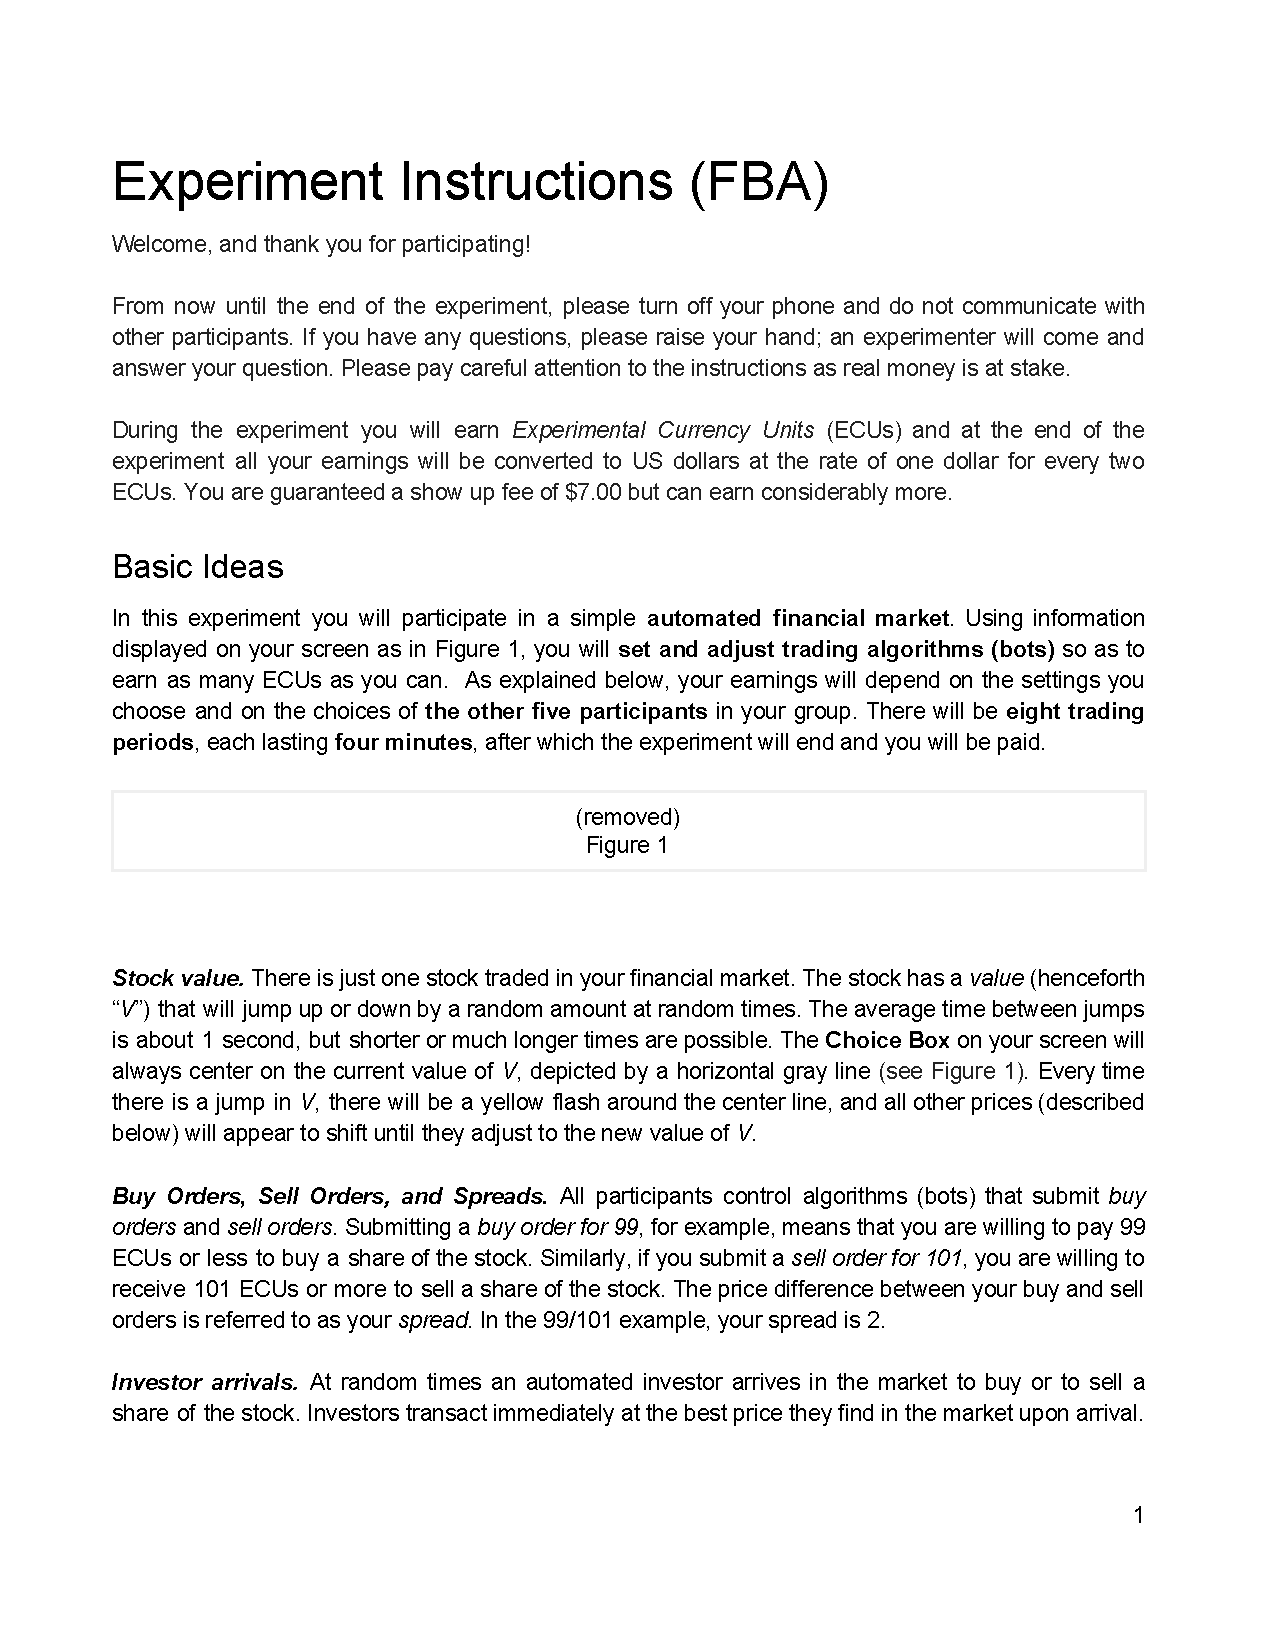
\includepdf[pages=-, pagecommand={}, scale=0.9]{CDA_instructions_for_paper1.pdf}

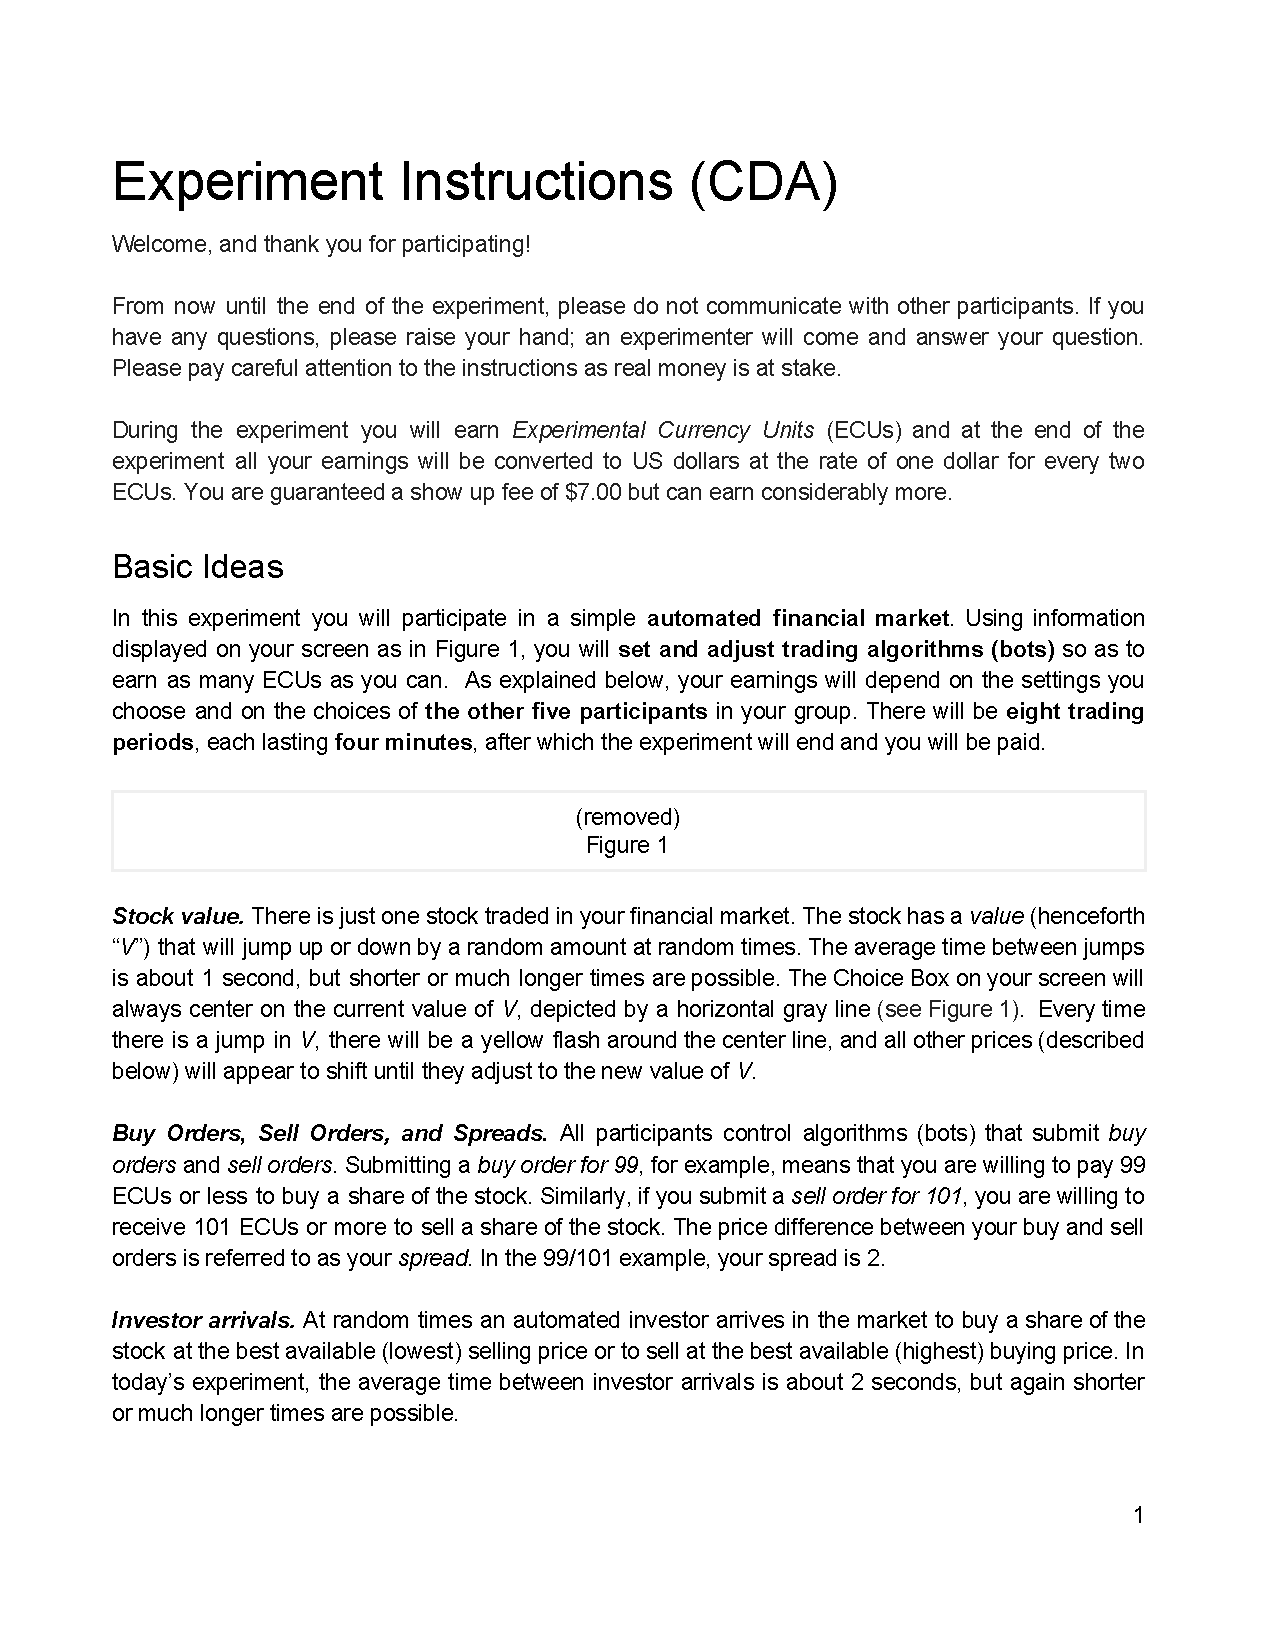
\includepdf[pages=-, pagecommand={}, scale=0.9]{FBA_instructions_for_paper1.pdf}

\end{appendices}

\end{document}

% TRANSACTIONS an 

\begin{table}
\centering
\caption{Transactions and RMSd}
\label{my-label}
\begin{tabular}{l|ccccc|cc}
\toprule
\multicolumn{8}{c}{CDA}                                                                                               \\
\multicolumn{1}{c}{} & Sys \# Trans & New \# Trans &                &                   &  & \multicolumn{2}{c}{RMSd - All} \\
Config 1             & 167.8        & 165.9        &                &                   &  &                & 0.3546  \\
Config 2             & 200.8438     & 199.1562     &                &                   &  &                & 0.5088  \\
Config 3             & 263.5938     & 257.5        &                &                   &  &                & 0.4665  \\
\midrule                    
\multicolumn{8}{c}{FBA}                                                                                               \\
\multicolumn{1}{c}{} & Sys \# Trans & New \# Trans & Invs' \# Trans & Traders' \# Trans &  & \multicolumn{2}{c}{RMSd}     \\
\multicolumn{1}{c}{} &              &              &                &                   &  & Only Traders;  & All \\
Config 1             & 103.7188     & 85.375       & 14.3438        & 71.0312           &  & 0.2447         & 0.2149  \\
Config 2             & 192.9375     & 104.125      & 5.875          & 98.25             &  & 0.4533         & 0.4278  \\
Config 3             & 186.6562     & 132.4062     & 22.2812        & 110.125           &  & 0.4603         & 0.377  \\
\bottomrule
\end{tabular}
\end{table}



